\chapter{RFD and MRAI correlation}
\label{cha:bgp_rfd}

%\begin{itemize}
%    \item Expose more deeply what is RFD
%    \item Expose previous studies about RFD
%    \item Today RFD? Outdated
%\end{itemize}

\ac{RFD} is another parameter of \ac{BGP} used to avoid messages storms.
It is used to avoid flapping routes to continuously make the network unstable.
When a network flaps a certain value is increased and when it overpass a threshold
then the route is suppressed and not advertised anymore until it goes back
below the threshold (or after a certain time).

\ac{RFD}, other than \ac{MRAI}, is one of the most studied parameters of \ac{BGP}
because of its influence in the convergence time \cite{mao2002route,pelsser2011route}.
\ac{RFD} received different updates from its first implementation, but recent 
studies showed that most of the providers still use outdated parameters \cite{gray2020bgp}.

The use of deprecated values can lead to a heavy restrictive suppression
of small routes delaying the correct spreading of information.
Some cases of suppression are caused by faulty interfaces that heavily flaps hundreds of times, 
while other times is just an update of the node configuration that
cause the route to flaps a couple of times and still be suppressed.

In the following chapters, I am going to show how legacy \ac{RFD} can affect 
small flaps and how would the new version of \ac{RFD} react to them.
Finally, I would look forward to understand the correlation between \ac{RFD}
and \ac{MRAI}.
When a suppressed route is shared again it could provoke messages storms that
triggers different \ac{MRAI} session, or the opposite case, a low \ac{MRAI} that
cause the growth of the figure of merit that suppresses a route.

\section{RFD on toy topologies}
\label{sec:bgp_rfd_toy}

I firstly studied \ac{RFD} on toy topologies, to see the effects of it in small 
networks, like I did in \Cref{sec:bgp_mrai_clique}.
As a graph, I used a clique of dimension \num{10}, the source of the signalling
is connected to the node \num{0} while the node \num{5} act as unique servicer
for the node $x$.
The node \num{5} won't be able to share information to node $x$ because of \ac{RFD}.
Node $x$ would have to wait until the route fell below the reuse threshold of 
node \num{5} to converge.

The parameters used for \ac{RFD} are the default \textit{CISCO} parameters,
showed in table \Cref{tbl:cisco_rfd}

\begin{table}[h]
	\begin{center}
	\begin{tabular}{ || m{5cm}| m{2cm} || } 
	\hline
	Parameter & Value \\ 
	\hline \hline
	withdrawal penalty & 1.0 \\
	\hline
    re-advertisement penalty & 0.0 \\
	\hline
    attribute change penalty & 1.0 \\
	\hline
    suppress threshold & 2.0 \\
	\hline
    half-life (min) & 15 (900s) \\
	\hline
    Reuse Threshold & 0.75 \\
	\hline
    Max Suppress Time (min.) & 60 (3600s) \\
	\hline
	\end{tabular}
\end{center}

	\caption{Cisco default \ac{RFD} parameters}
	\label{tbl:cisco_rfd}
\end{table}

The parameters of the environment are in \Cref{tbl:clique_rfd_params}

\begin{table}[h]
	\begin{center}
	\begin{tabular}{ || m{4cm}| m{8cm} || } 
	\hline
	Property & Value \\ 
	\hline \hline
	Seeds & $[1, 10]$ \\ 
	\hline
	Signaling & \q{AWAWAWA} \\
	\hline
		Withdraws delay & Constant distribution of \SI{300}{\second} \\ 
	\hline
	Announcement delay & constant distribution of \SI{300}{\second} \\ 
	\hline
		MRAI & $[0, 120]$ \\
	\hline
	Link delay & Uniform distribution between \SI{0.012}{\second} and \SI{3}{\second} \\
	\hline
	\end{tabular}
\end{center}

	\caption{Environment parameters used for the experiments on \ac{RFD}
		with the clique graph}
	\label{tbl:clique_rfd_params}
\end{table}

Messages in the signal are delayed by \SI{300}{\second} for two reasons:
\begin{itemize}
	\item The main goal of these experiments is to study the correlation from
		\ac{RFD} to \ac{MRAI} and we don't want that \ac{MRAI} compress
		parts of the signal.
	\item I'm trying to simulate one of the possible behaviour tat triggers
		\ac{RFD} suppressions, the human faulty reconfiguration of the node.
\end{itemize}

The signals contain \num{3} flaps in it, the first one is hipotetically attributed
to a configuration that doesn't work properly, the second one is caused by a
buggy correction of the configuration and the last one by the introduction of a
correct configuration.

The \ac{MRAI} strategy used in all the experiments is the \textit{fixed} one.

\begin{figure}[h]
     \centering
     \begin{subfigure}[b]{0.45\textwidth}
         \centering
		 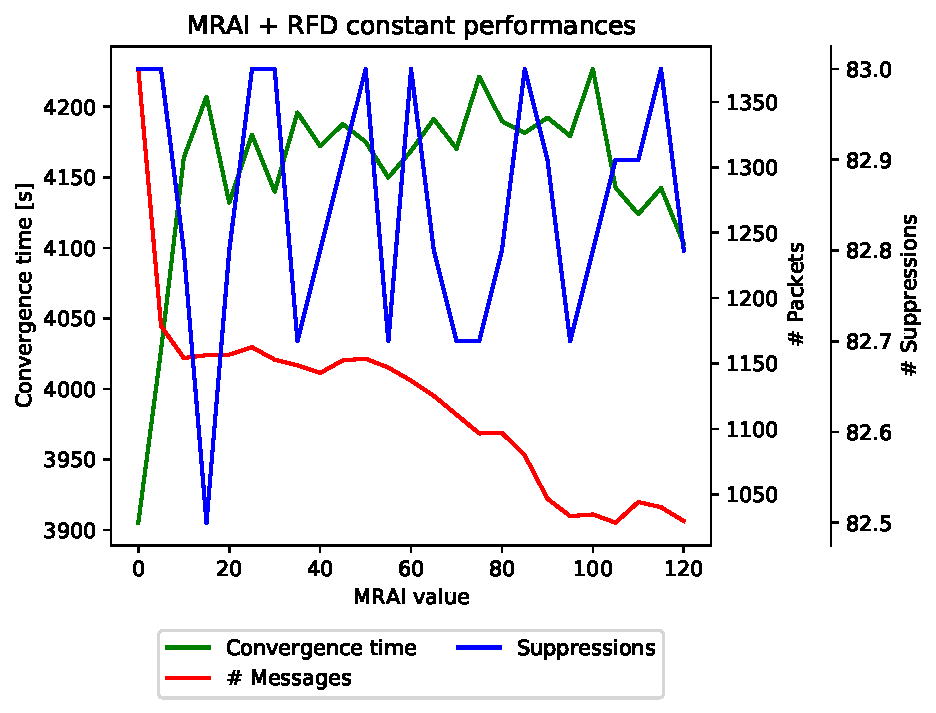
\includegraphics[width=\textwidth]{images/RFD/clique/cisco_clique10_RFD-constant_mrai_rfd_evolution.pdf}
		 \caption{Network performances with the standard cisco \ac{RFD}}
		 \label{fig:clique_evolution_rfd}
     \end{subfigure}
     \hfill
     \begin{subfigure}[b]{0.45\textwidth}
         \centering
         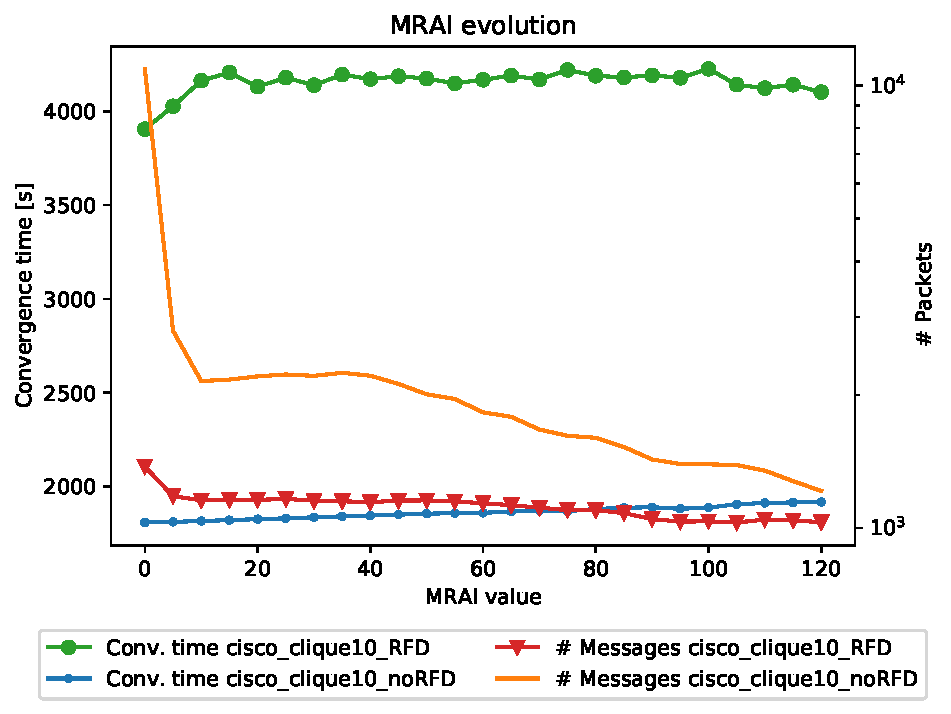
\includegraphics[width=\textwidth]{images/RFD/clique/cisco_clique10_comparison_constant_all.pdf}
		 \caption{Network performances standard \ac{RFD} vs no \ac{RFD}}
         \label{fig:clique_evolution_rfd_vs_noRFd_comparison}
     \end{subfigure}
		\caption{Evolution of the performances changing \ac{MRAI} in the links
			standard \ac{RFD} vs no \ac{RFD},
			graph clique of \num{10} nodes, \ac{MRAI} strategy fixed, signal \q{AWAWAWA}}
        \label{fig:clique_evolution_rfd_vs_noRFD}
\end{figure}

The plot in \Cref{fig:clique_evolution_rfd} contains a third line that represent 
the total number of suppressions detected on the experiment, for each experiment
has been executed \num{10} different runs.
The blue line that represents the number of suppressions refers to the third y-axis
on the right.

In \cref{fig:clique_evolution_rfd} is possible to see that small changes to \ac{MRAI}
can lead to some differences in the number of suppressions.
Also, the number of messages decreases rapidly and reaches a constant 
value around 980, as expected by the passage from an \ac{MRAI} of \SI{0}{\second}
to a few seconds.
The nodes that don't trigger a suppression seems to affect also the
convergence time that grows as expected but with a lot of fluctuations.

In \Cref{fig:clique_evolution_rfd_vs_noRFd_comparison} is possible to see the
gap between the use of \ac{RFD} and without it.
Notice that the packet axis is in log scale.
The difference in the convergence time is due to the fact that with \ac{RFD} some
nodes block the best path that takes a lot of time to become available again.
While \ac{MRAI} grows the set of nodes that suppress routes decreases but the
convergence time is highly affected by a restrict subset of them.
In our case, for example, the suppressions on nodes \num{0} and \num{5} plays
an important role.
The first one for the spreading in the whole network, the second one for the
transmission of information to node $x$.

For this reason, we can look more deeply on what happened to the figure of merit
of node $x$ and five in \Cref{fig:clique_nodex,fig:clique_node5}

\begin{figure}[h]
     \centering
     \begin{subfigure}[b]{0.3\textwidth}
         \centering
         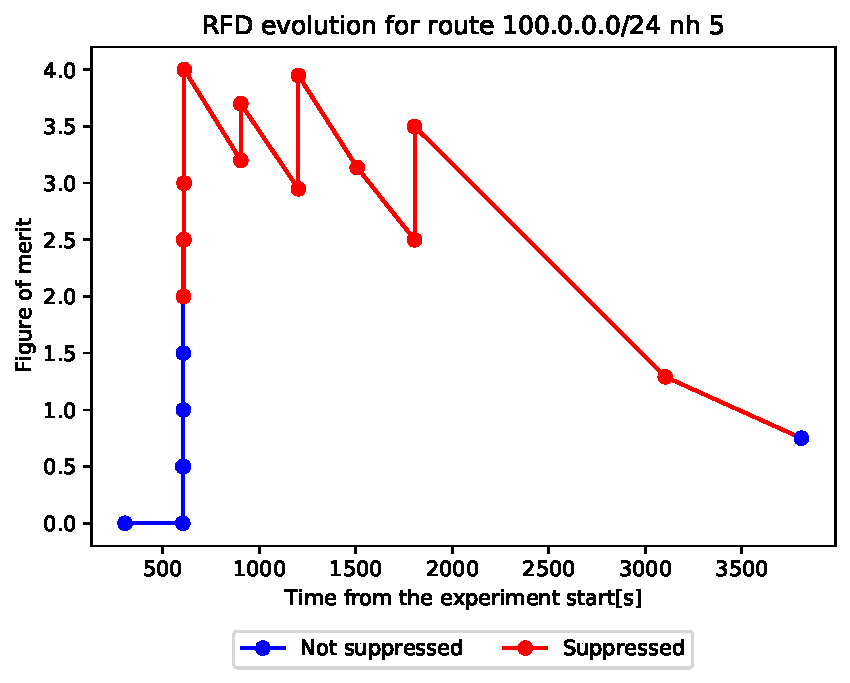
\includegraphics[width=\textwidth]{images/RFD/clique/FigureOfMerit/mrai1_RFD_x_rfd_R1.pdf}
         \caption{MRAI = 0s}
         \label{fig:clique_x_mrai0}
     \end{subfigure}
     \hfill
     \begin{subfigure}[b]{0.3\textwidth}
         \centering
         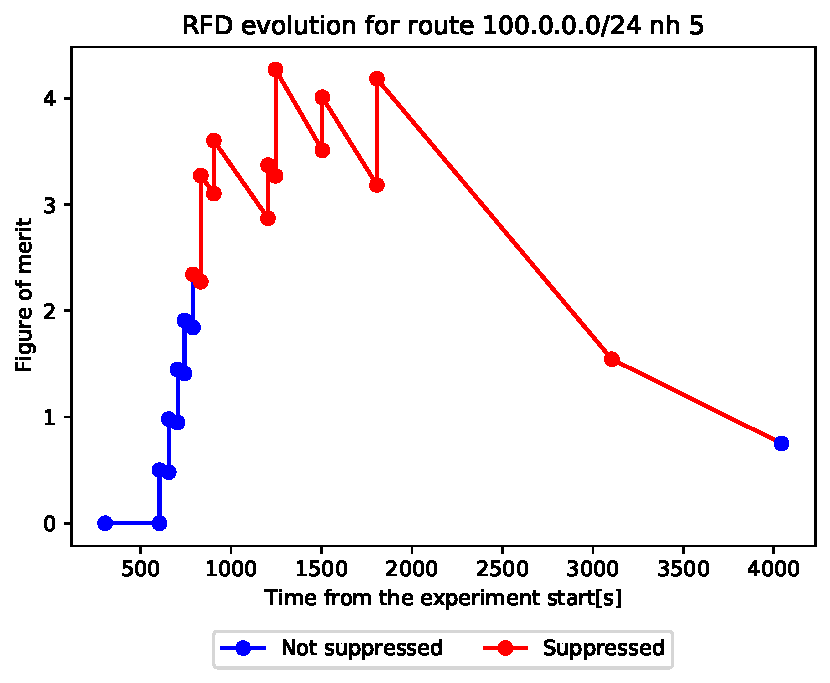
\includegraphics[width=\textwidth]{images/RFD/clique/FigureOfMerit/mrai11_RFD_x_rfd_R1.pdf}
         \caption{MRAI = 50s}
         \label{fig:clique_x_mrai50}
     \end{subfigure}
     \hfill
     \begin{subfigure}[b]{0.3\textwidth}
         \centering
         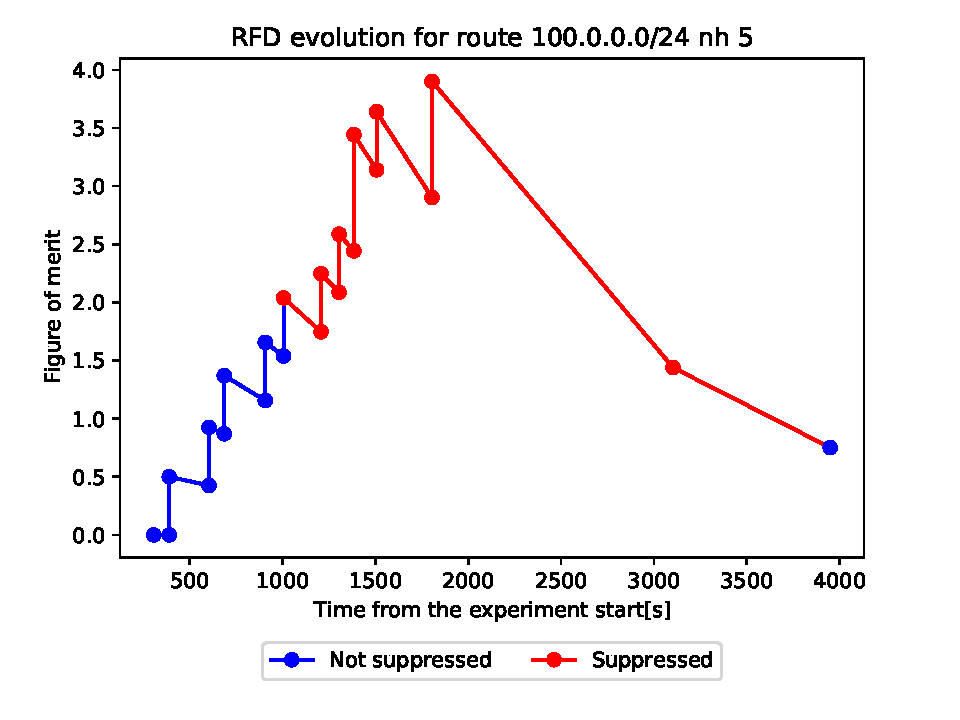
\includegraphics[width=\textwidth]{images/RFD/clique/FigureOfMerit/mrai21_RFD_x_rfd_R1.pdf}
         \caption{MRAI = 100s}
         \label{fig:clique_x_mrai100}
     \end{subfigure}
        \caption{Evolution of the figure of merit in the node X with different MRAIs}
        \label{fig:clique_nodex}
\end{figure}

The node $x$ is a leaf of the network that will absorb everything the node \num{5}
sends to it.
In \Cref{fig:clique_nodex} is possible to see the evolution of the figure of merit
with different \ac{MRAI} values.
In the first case, with an \ac{MRAI} qual to \SI{0}{\second}, we will see a huge
spike caused bt a lot of messages and route changes that the node \num{5} sends
to it.
while in the other two cases \Cref{fig:clique_x_mrai50,fig:clique_x_mrai100} 
the \ac{MRAI} seems to not be much effective on the route through node \num{5}.
In those cases, we can see that the route has been suppressed around \SI{1000}{\second}
and is going to become useful again around \SI{4000}{\second}.
In this period of time from \SI{1000}{\second} to \SI{4000}{\second}, it still
receives some updates from node \num{5} that changes its own best path, and this
makes the figure of merit evolve.
The evolution of the figure of merit stops around \SI{2000}{\second} that's because
also the node \num{5} has suppressed the route, \Cref{fig:clique_node5}.
The point around \SI{3000}{\second} represent the moment when the route becomes
available again for node \num{5} that communicates the change to $x$.

\begin{figure}[h]
     \centering
     \begin{subfigure}[b]{0.3\textwidth}
         \centering
         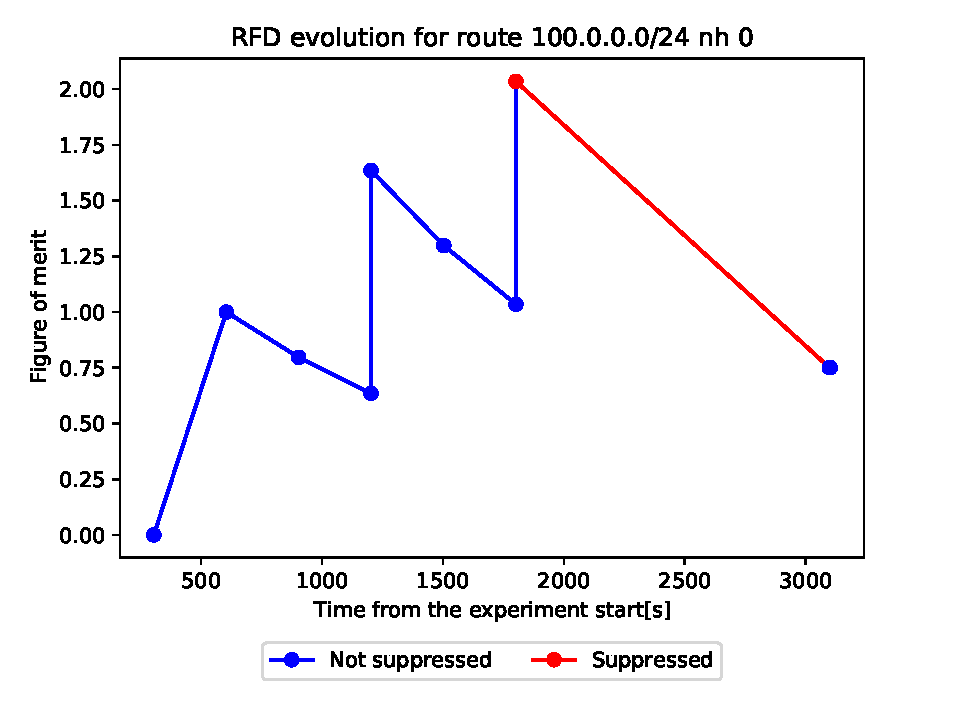
\includegraphics[width=\textwidth]{images/RFD/clique/FigureOfMerit/mrai1_RFD_5_rfd_R1.pdf}
         \caption{MRAI = 0s}
         \label{fig:clique_5_mrai0}
     \end{subfigure}
     \hfill
     \begin{subfigure}[b]{0.3\textwidth}
         \centering
         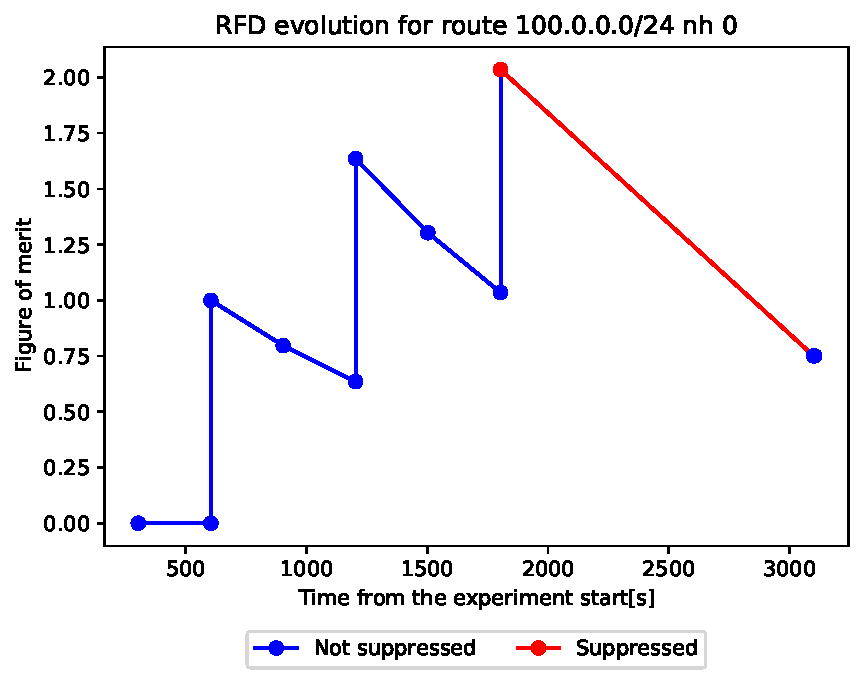
\includegraphics[width=\textwidth]{images/RFD/clique/FigureOfMerit/mrai11_RFD_5_rfd_R1.pdf}
         \caption{MRAI = 50s}
         \label{fig:clique_5_mrai50}
     \end{subfigure}
     \hfill
     \begin{subfigure}[b]{0.3\textwidth}
         \centering
         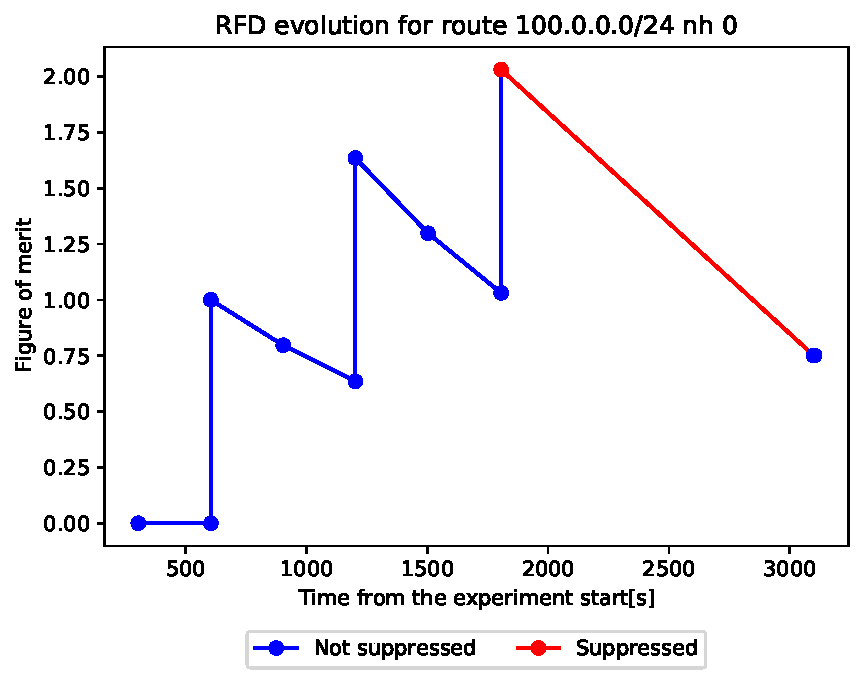
\includegraphics[width=\textwidth]{images/RFD/clique/FigureOfMerit/mrai21_RFD_5_rfd_R1.pdf}
         \caption{MRAI = 100s}
         \label{fig:clique_5_mrai100}
     \end{subfigure}
        \caption{Evolution of the figure of merit in the node X with different MRAIs}
        \label{fig:clique_node5}
\end{figure}

The evolution of the figure of merit of the best path of node \num{5} is a different
from the one of node $x$.
In fact, it is not influenced by \ac{MRAI} as we can see in \Cref{fig:clique_node5}.
That because the node \num{5} us directly connected to the node \num{0} that every
\SI{300}{\second} forward the message of $d$ and \SI{300}{\second} is delay 
too large to be affected by the compression effect of \ac{MRAI}.
Around \SI{2000}{\second} node \num{5} suppress the route (as any other node in the
clique) and stops to forward it to node $x$ until \SI{3000}{\second} when it become
available again.

Node $x$ took almost \SI{4000}{\second} to converge because of the big fluctuations
of node \num{5} that suffers of the \textit{Path Exploration} problem, the path
changes are considered bad behaviour in \ac{RFD}.

In conclusion, we can say that \ac{RFD} can be affected by \ac{MRAI} and
that \ac{RFD} can prevent a lot of messages at the cost of very high convergence
times.

%\begin{itemize}
%    \item What is the impact of RFD?
%    \item In which occasion is present RFD?
%    \item Clique
%    \item Variations thanks to MRAI
%\end{itemize}

\section{RFC 2439 VS RFC 7196}
\label{sec:bgp_rfd_comparison}

The difference in the two \ac{RFC} that defines \ac{RFD} \cite{rfc2439,rfc7196}
is in the parameters used.
Infact the last \ac{RFC} introduced two new set of parameters where the figure
of merit threshold is increased up to at least \num{6.0}.
The two category are:
\begin{itemize}
	\item \textit{\textbf{Aggressive}}, Suppression threshold no less than \num{6.0};
	\item \textit{\textbf{Conservative}}, Suppression threshold no less than \num{12.0};
\end{itemize}

Respectively \num{3} and \num{6} times the actual standard.

I have then repeated the same experiments of \Cref{sec:bgp_rfd_toy} with the same
clique graph, but with the two new \ac{RFD} strategies, the results are 
showed in \Cref{fig:clique_rfd7196}.

\begin{figure}[h]
     \centering
     \begin{subfigure}[b]{0.48\textwidth}
         \centering
         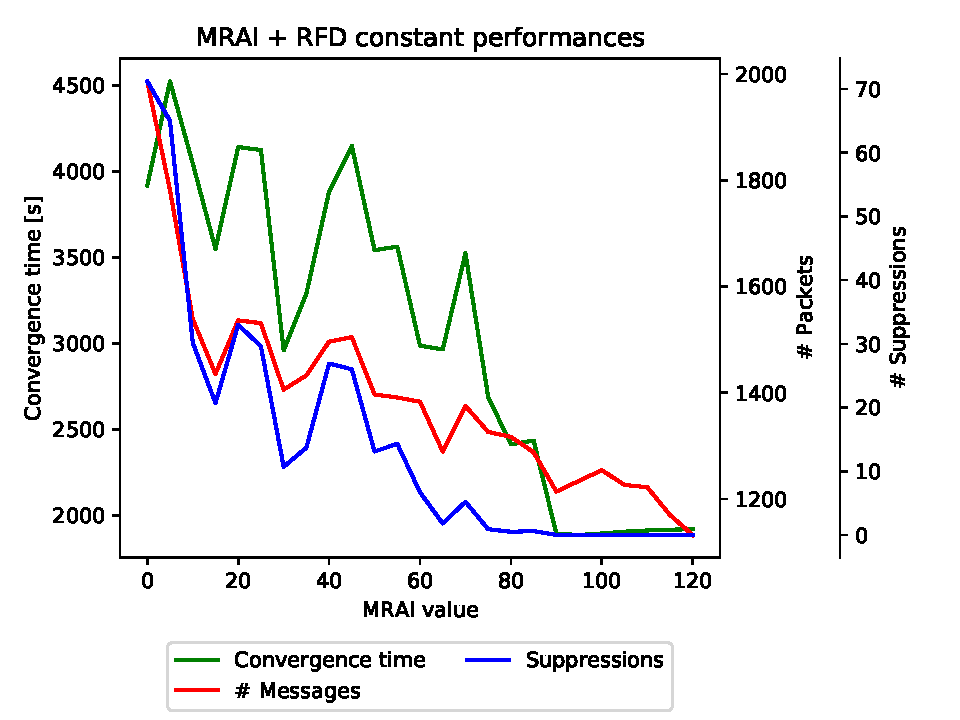
\includegraphics[width=\textwidth]{images/RFD/clique/cisco_clique10_RFD_7196_aggressive-constant_mrai_rfd_evolution.pdf}
         \caption{RFD 7196 Aggressive on the clique topology}
         \label{fig:rfd7196aggressive}
     \end{subfigure}
     \hfill
     \begin{subfigure}[b]{0.48\textwidth}
         \centering
         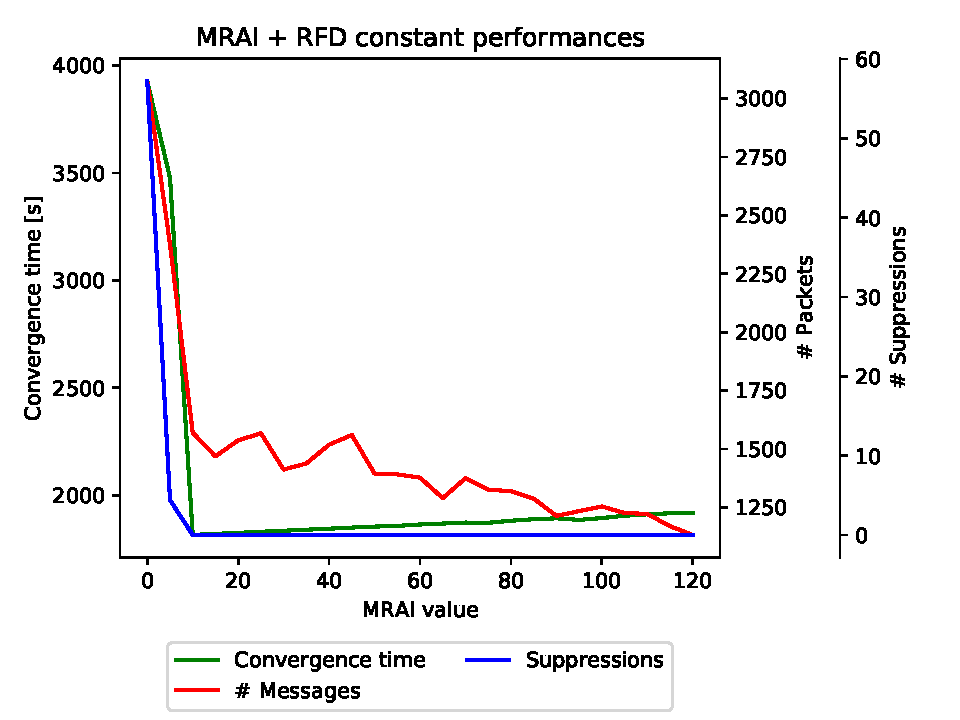
\includegraphics[width=\textwidth]{images/RFD/clique/cisco_clique10_RFD_7196_conservative-constant_mrai_rfd_evolution.pdf}
         \caption{RFD 7196 Conservative on the clique topology}
         \label{fig:rfd7196conservative}
     \end{subfigure}
		\caption{MRAI influence with different RFD strategies from \cite{rfc7196}}
        \label{fig:clique_rfd7196}
\end{figure}

We can see two completely different evolutions of the performances in \Cref{fig:clique_rfd7196}.
On the left plot, we can see the evolution with the \textit{Aggressive} strategy.
and \ac{MRAI} is more effective to this strategy in respect of the standard one.
The number of suppressions fell down to almost \num{0} with an \ac{MRAI} near 
\SI{90}{\second}.
The message trend is similar to the one of the case without \ac{RFD} but with an
important difference in the case of  \ac{MRAI} equal \SI{0}{\second}, the number
of average messages is around \num{2000} in respect of the \num{6000} without
\ac{RFD}.
While with a high \ac{MRAI} the message trends are similar and equal when the number of
suppressions reaches \num{0}.

The convergence time, on the other hand, has the opposite trend in respect of 
the one that we saw in \Cref{fig:clique_evolution_rfd}.
Here we see a descending trend caused by the fact that \ac{MRAI} is able to avoid
some messages and, as a consequence, avoid the growing of the figure of merit in 
some nodes permitting to the convergence time to decrease.
Once the number of suppressions reaches \num{0} obviously the network performances
are equal as in the \textit{NoRFD} case.

In \Cref{fig:rfd7196conservative} we can see the evolution of the network with the 
\textit{Conservative} strategy, the threshold of this strategy is the double of
the \textit{Aggressive} strategy.
The effects of this difference are huge, is sufficient an \ac{MRAI} of \SI{10}{\second}
to avoid at all suppressions, causing the trend, in terms of messages and
convergence time as if there is no \ac{RFD} at all.
Also with an \ac{MRAI} of \SI{0}{\second} is possible to see a difference in 
terms of messages and convergence time in respect of the other two strategies.
This is the strategy that more likely resembles the \textit{NoRFD} one,
having a convergence time incredibly more low, at the cost of few hundreds messages.

We can now take a look more closely to what happens to the figure of merit 
for the only route that node $x$ receives.
Results are exposed in \Cref{fig:clique_nodex_rfd7196Aggressive}

\begin{figure}[h]
     \centering
     \begin{subfigure}[b]{0.3\textwidth}
         \centering
         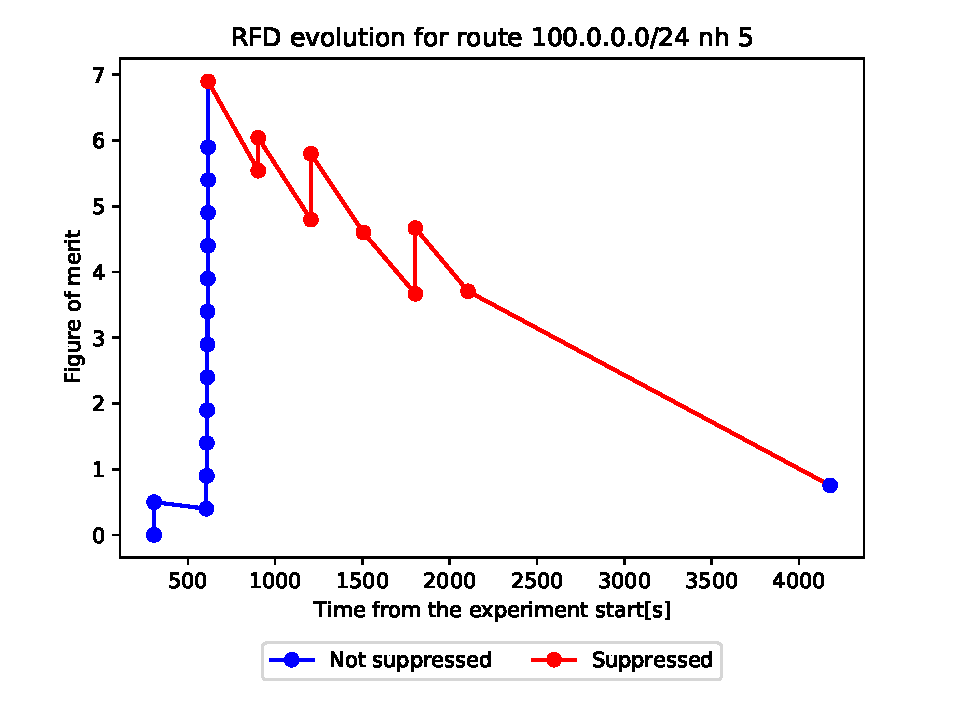
\includegraphics[width=\textwidth]{images/RFD/clique/FigureOfMerit/mrai1_RFD_7196_aggressive_x_rfd_R1.pdf}
         \caption{MRAI = 0s, RFD 7196 Aggressive, clique topology}
         \label{fig:clique_x_mrai0_rfd7196Aggressive}
     \end{subfigure}
     \hfill
     \begin{subfigure}[b]{0.3\textwidth}
         \centering
         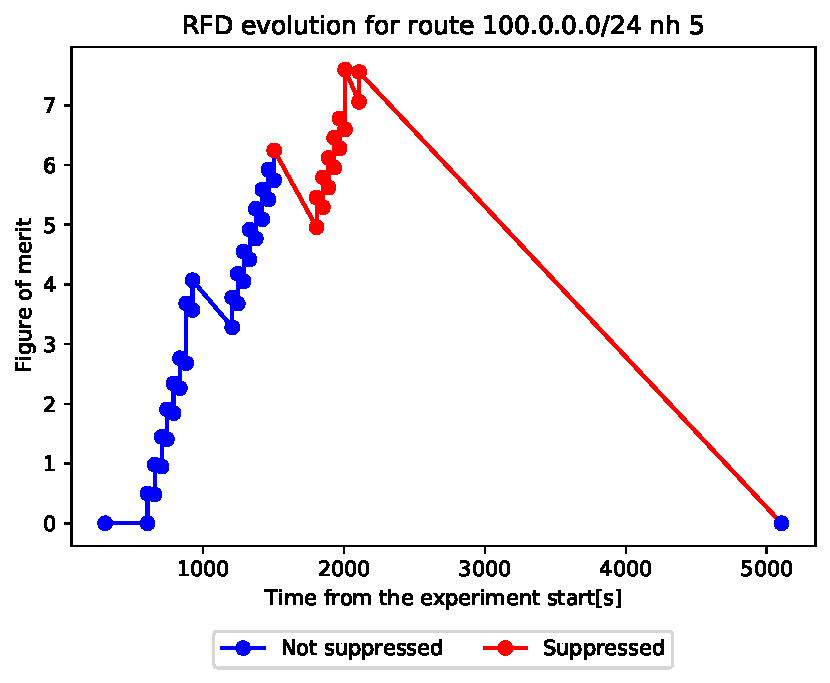
\includegraphics[width=\textwidth]{images/RFD/clique/FigureOfMerit/mrai11_RFD_7196_aggressive_x_rfd_R1.pdf}
         \caption{MRAI = 50s, RFD 7196 Aggressive, clique topology}
         \label{fig:clique_x_mrai50_rfd7196Aggressive}
     \end{subfigure}
     \hfill
     \begin{subfigure}[b]{0.3\textwidth}
         \centering
         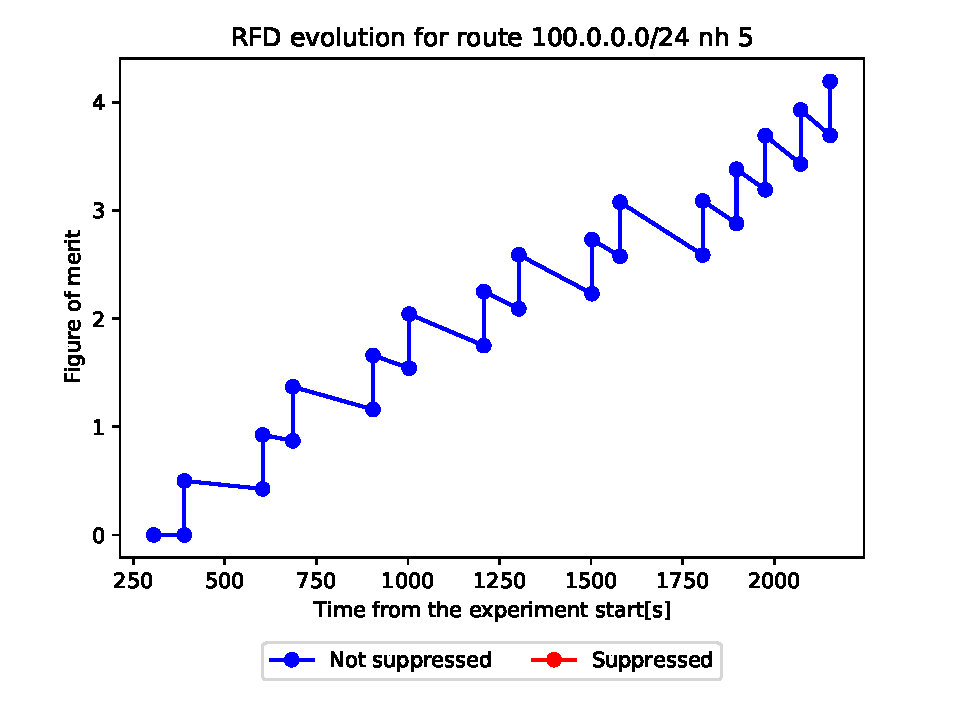
\includegraphics[width=\textwidth]{images/RFD/clique/FigureOfMerit/mrai21_RFD_7196_aggressive_x_rfd_R1.pdf}
         \caption{MRAI = 100s, RFD 7196 Aggressive, clique topology}
         \label{fig:clique_x_mrai100_rfd7196Aggressive}
     \end{subfigure}
        \caption{Evolution of the figure of merit in the node X with different MRAIs, with RFD 7196 aggressive in a clique topology}
        \label{fig:clique_nodex_rfd7196Aggressive}
\end{figure}

We can see in \Cref{fig:clique_x_mrai0_rfd7196Aggressive,fig:clique_x_mrai50_rfd7196Aggressive}
that \ac{MRAI} plays an important role in the figure of merit of node $x$.
In the first case, the route would be delayed up to \SI{4000}{\second} while
in the second one, the grow never touches the threshold.
We can also notice that there is a small difference in the growth with a higher
\ac{MRAI}, in \Cref{fig:clique_x_mrai100_rfd7196Aggressive} we can notice a 
slower grow, thanks to the fact that node \num{5} has to send a smaller amount
of messages to correct its knowledge.

In conclusion, if before \ac{MRAI}, with the standard \ac{RFD} was playing a more
marginal role because of the restrictive threshold, now, with those strategies
it can play a more relevant role and act as a key factor between the suppression 
or not.

%\begin{itemize}
%    \item Time comparison between both of them
%    \item how them react differently?
%    \item why?
%\end{itemize}

\section{Mice VS Elephants}
\label{sec:bgp_rfd_mice_vs_elephants}

From the work of R. Bush et al., \cite{pelsser2011route} we know that the majority
of updates that are transmitted on the Internet are from a small set of \ac{AS}.
Those \ac{AS}es with their flaps causes update storms almost continuously.
I report a figure from \cite{pelsser2011route} for simplicity in 
\Cref{fig:RBushPrefixes}
Thanks to the studies of APNIC \fxfatal{insert citation of footnote, something}
we also know that this behaviour is still present nowadays, the \Cref{fig:apnicPrefixes}
is taken from one of their annual reports and shows that the \num{10}\% of
all the active prefixes produce more or less the \num{70}\% of the total
updates.

\begin{figure}[h]
     \centering
     \begin{subfigure}[b]{0.48\textwidth}
         \centering
         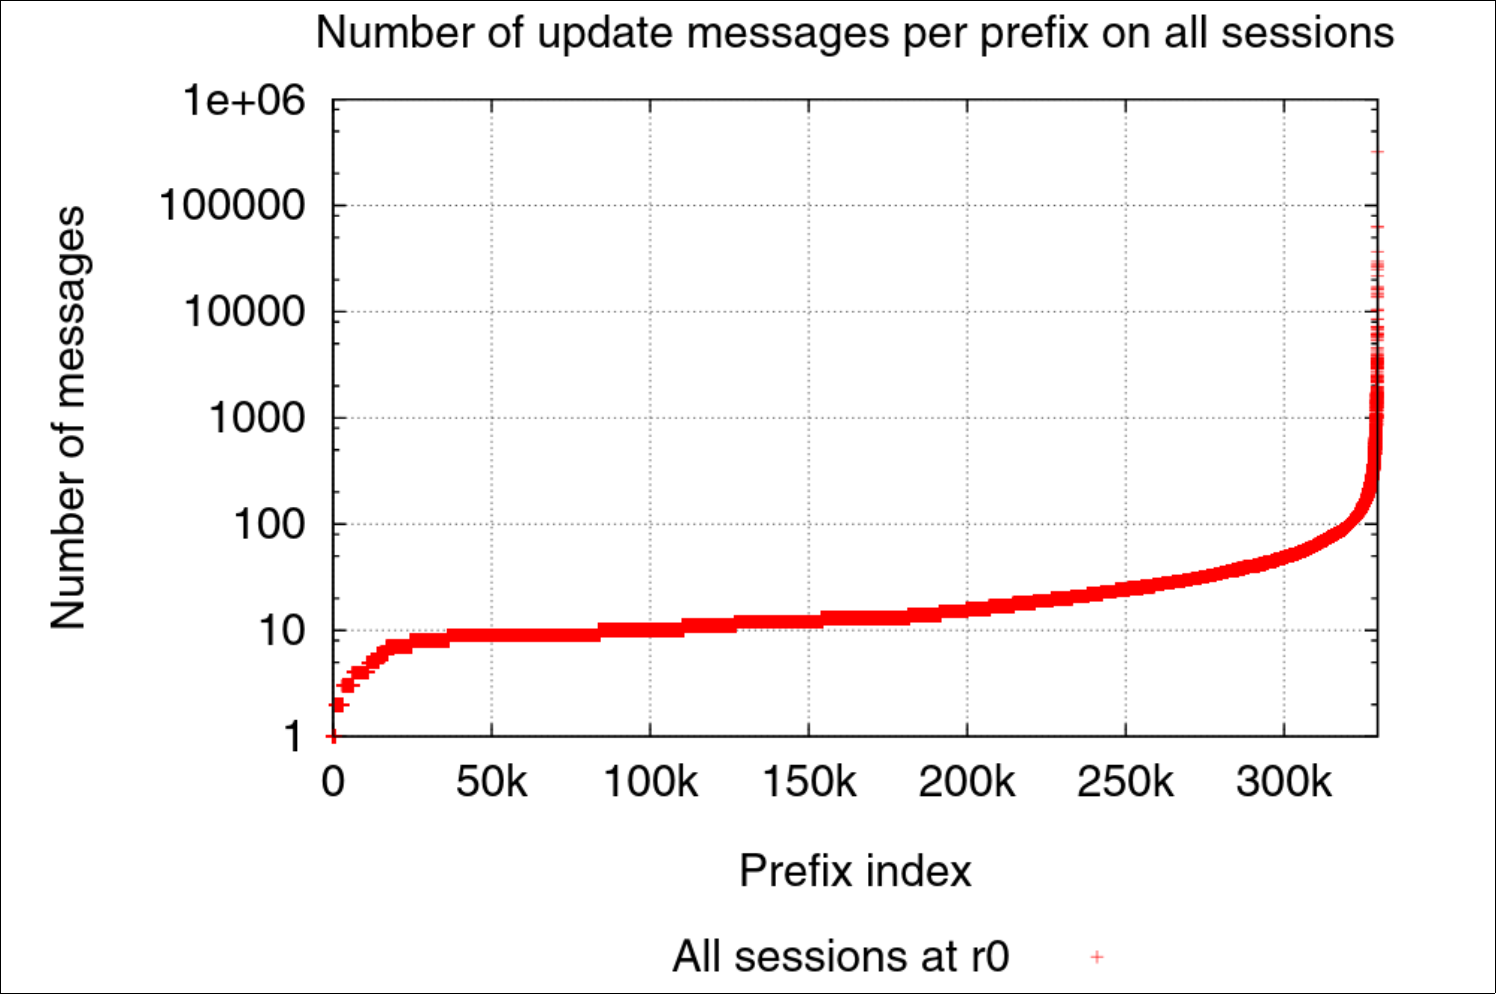
\includegraphics[width=\textwidth]{images/RFD/miceVSelephants/prefixVSmessagesRbush.png}
		 \caption{Prefixes and number of updates associated, figure from \cite{pelsser2011route}}
         \label{fig:RBushPrefixes}
     \end{subfigure}
     \hfill
     \begin{subfigure}[b]{0.48\textwidth}
         \centering
         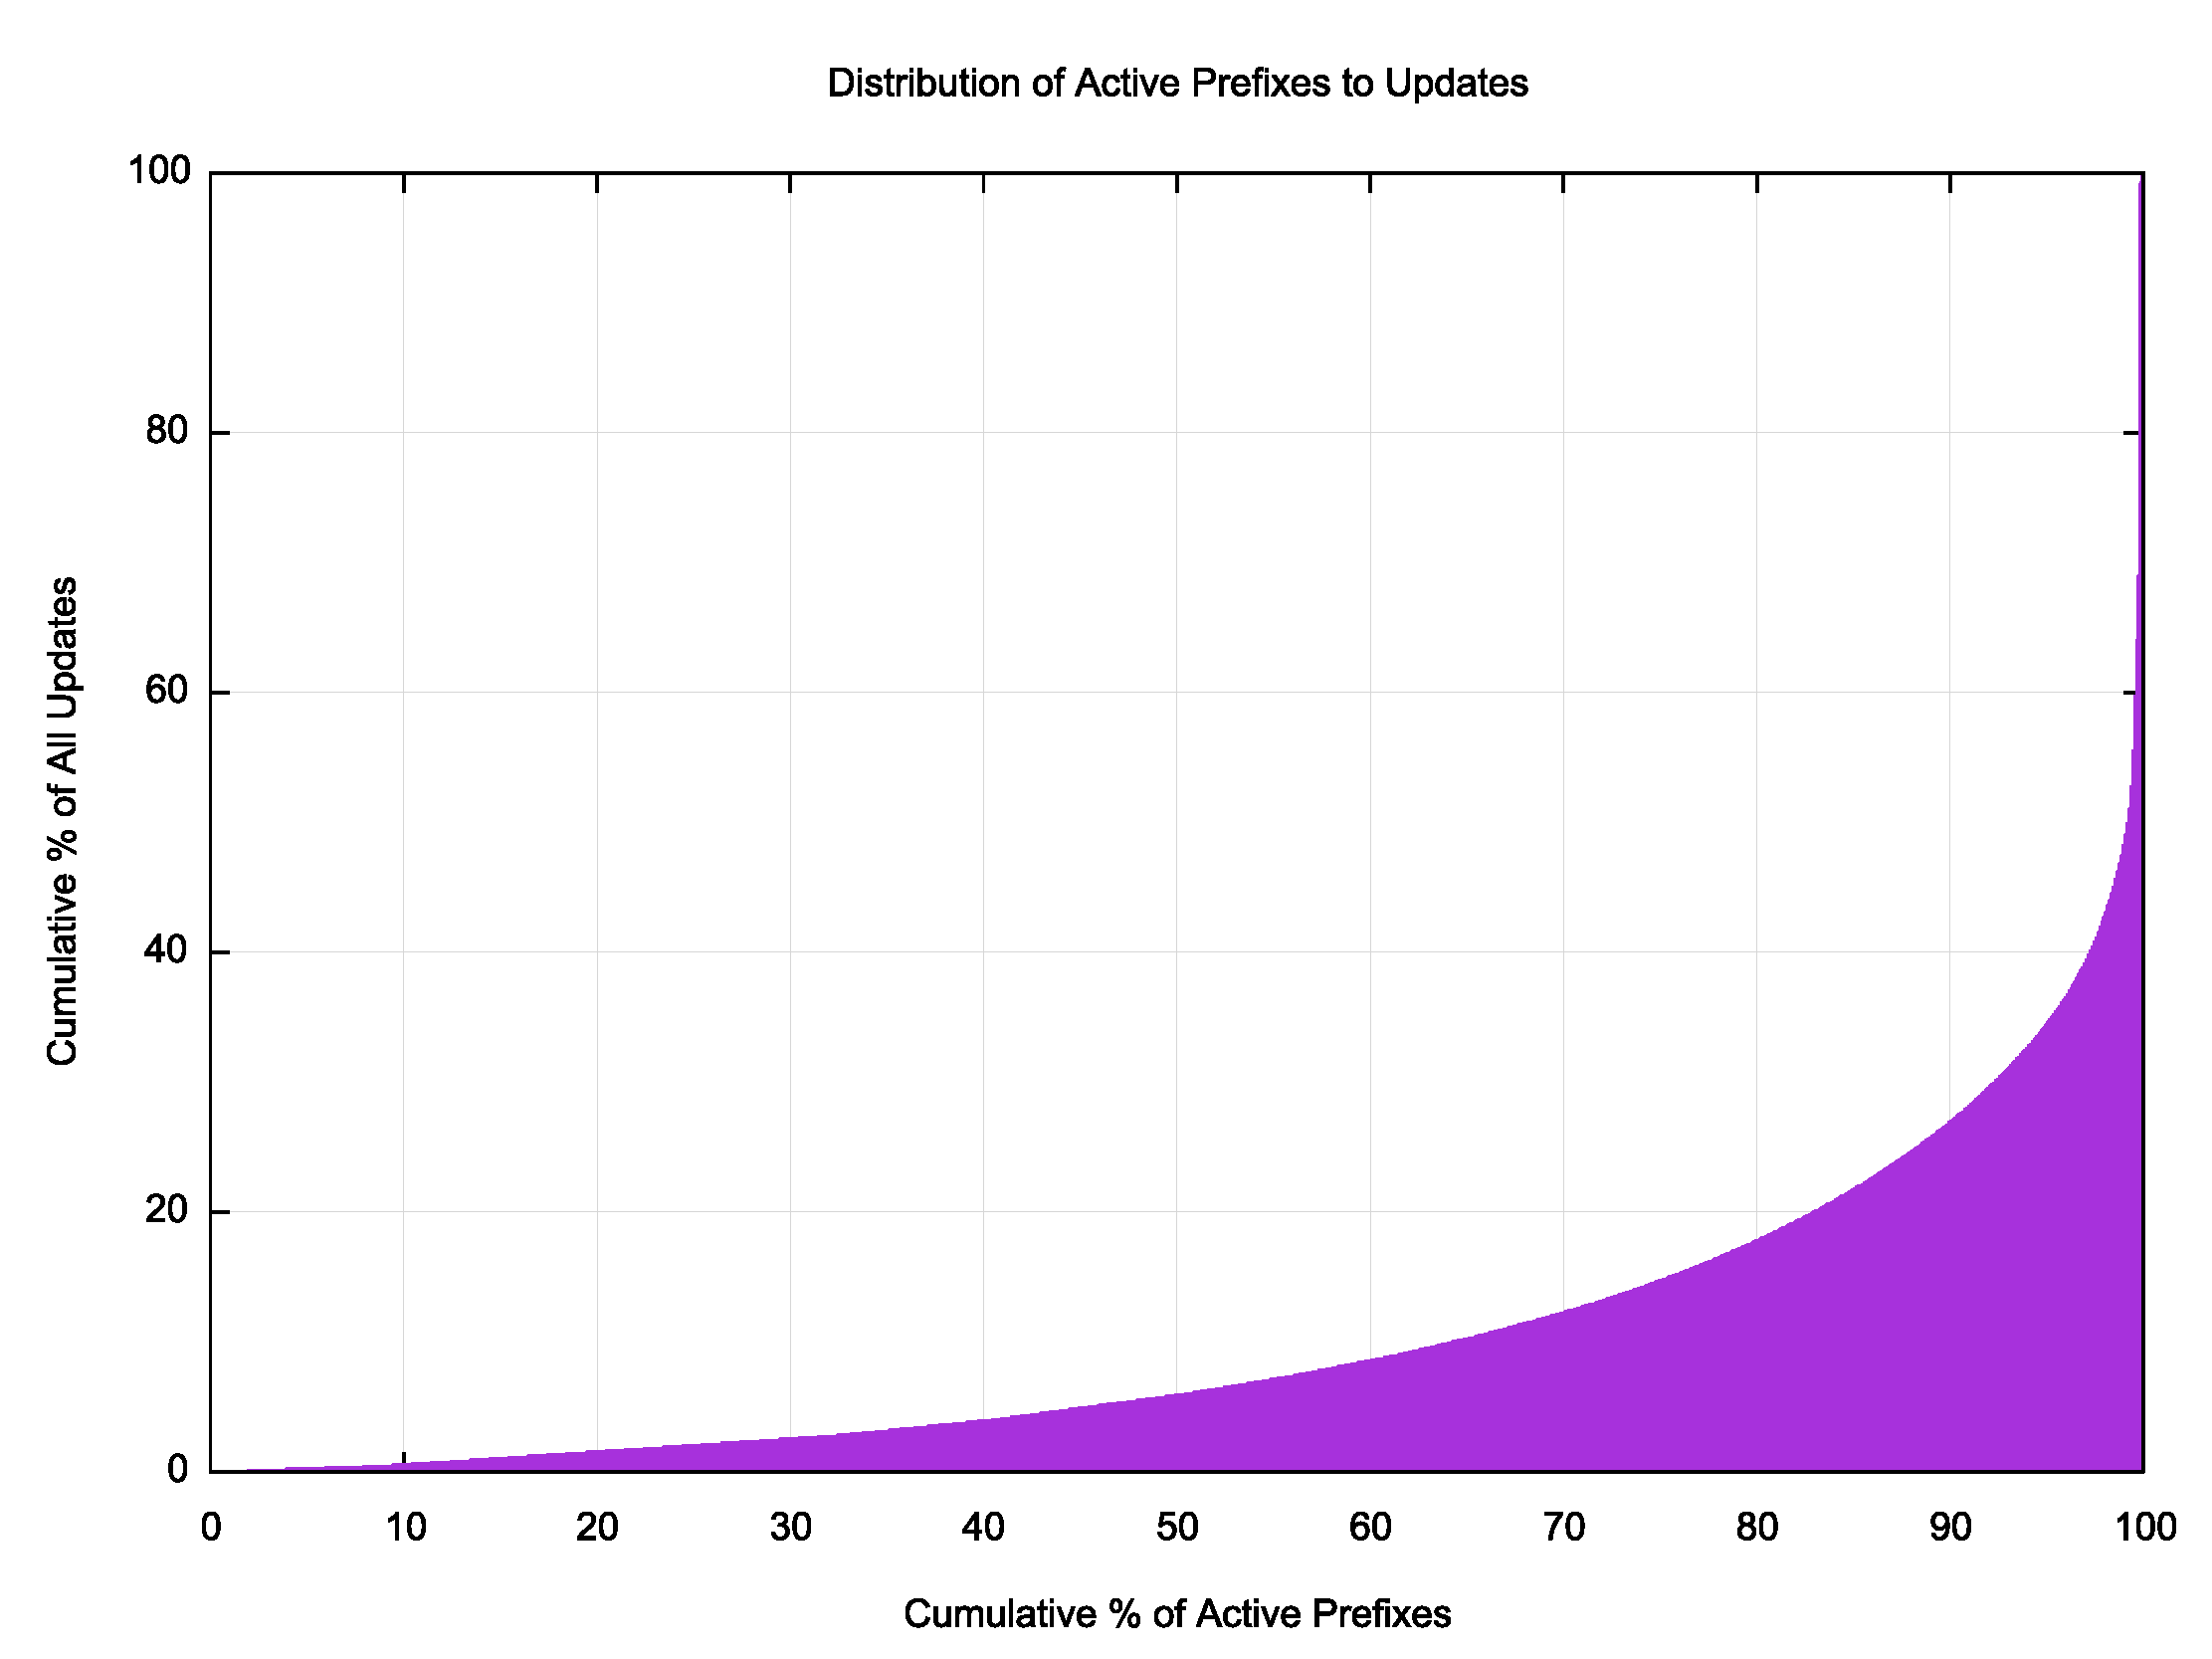
\includegraphics[width=\textwidth]{images/RFD/miceVSelephants/bgp2fig5-pfx-upds-cuml.png}
         \caption{Prefixes and number of updates associated, [apnic 2019]}
         \label{fig:apnicPrefixes}
     \end{subfigure}
        \caption{Prefixes influence on updates}
        \label{fig:prefixVSmessages}
\end{figure}

We can then divide those prefixes in two sets:
\begin{itemize}
	\item \textbf{\textit{Mice}}, this set represent the majority of the prefixes,
		all the prefixes that does not generate more than \num{100} updates 
		in \Cref{fig:RBushPrefixes}
	\item \textbf{\textit{Elephants}}, this set represent the remaining part
		of the prefixes, those that produces the majority of the messages.
\end{itemize}

Thanks to a review of a \ac{BGP} year by APNIC, presented at RIPE 52 \cite{huston2006bgp}, we can also have an example of those elephants prefixes.
This example is shown in \Cref{fig:ripePrefixFlaps}, it takes in consideration the
prefix \q{202.64.49.0/24} showing that in a relatively small period of time it has
produced thousands of \ac{ADV} per day.
In this case, this particular prefix has produced \num{198,370} \ac{ADV} producing
in total \num{96,330} flaps.

\begin{figure}[h]
    \centering
    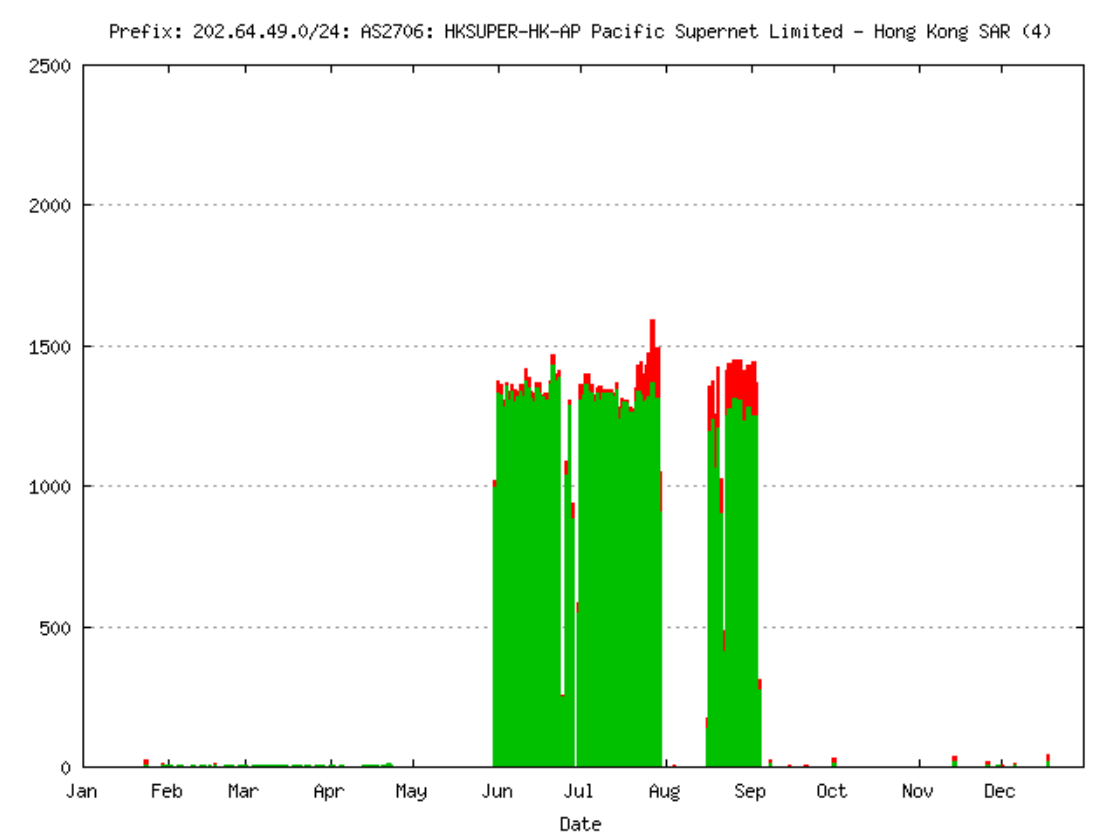
\includegraphics[scale=0.22]{images/RFD/miceVSelephants/ripePrefixFlap.png}
	\caption{202.64.49.0/24 flaps plot from \cite{huston2006bgp}}
    \label{fig:ripePrefixFlaps}
\end{figure}

I have then used this data to configure two new environments for the simulations.
The first one that points to reproduce the \textit{Mice} behaviour, the second
one the \textit{Elephants}.

In both these environments, I have then compared the four different strategies of
\ac{RFD}, \textit{NoRFD}, standard \ac{RFD} and the two from \cite{rfc7196}.

The topology used for those experiments is an \textit{Internet like} topology
with \num{1000} nodes and \ac{MRAI} is fixed to \SI{30}{\second} for all the links.
The source of the signal has been chosen randomly on the graph.
For each experiment has been then executed \num{50} runs.

\subsection{Mice}
\label{subsec:mice}

The particularity of the \textit{Mice} experiments is in the signal, we have
a low number of flaps interleaved by a long timer.
I have then used a signal with \num{5} flaps, \q{AWAWAWAWAWA} with a delay
of \SI{300}{\second} (\SI{5}{\minute}) between each message.
The results are presented in \Cref{fig:1000_RFD_MRAI30_mice}.

\begin{figure}[h]
     \centering
     \begin{subfigure}[b]{0.325\textwidth}
         \centering
         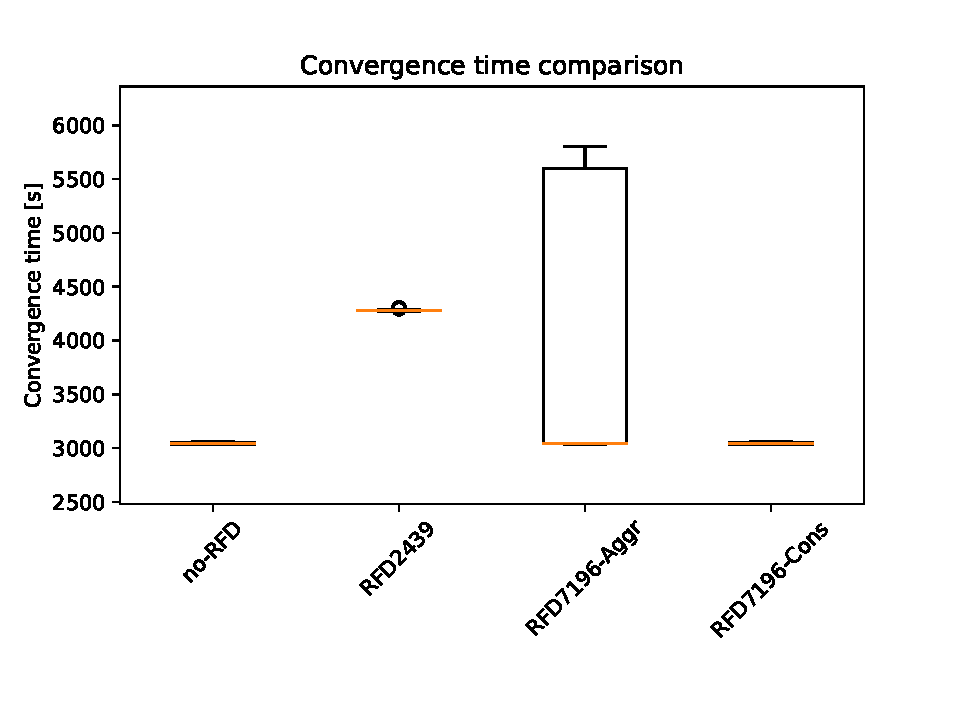
\includegraphics[width=\textwidth]{images/RFD/miceVSelephants/mice/cisco_1000MRAI30_rfd_comparison_time_boxplot.pdf}
         \caption{Convergence time respect to the RFD strategy}
         \label{fig:1000_RFD_MRAI30_mice_time}
     \end{subfigure}
     \hfill
     \begin{subfigure}[b]{0.325\textwidth}
         \centering
         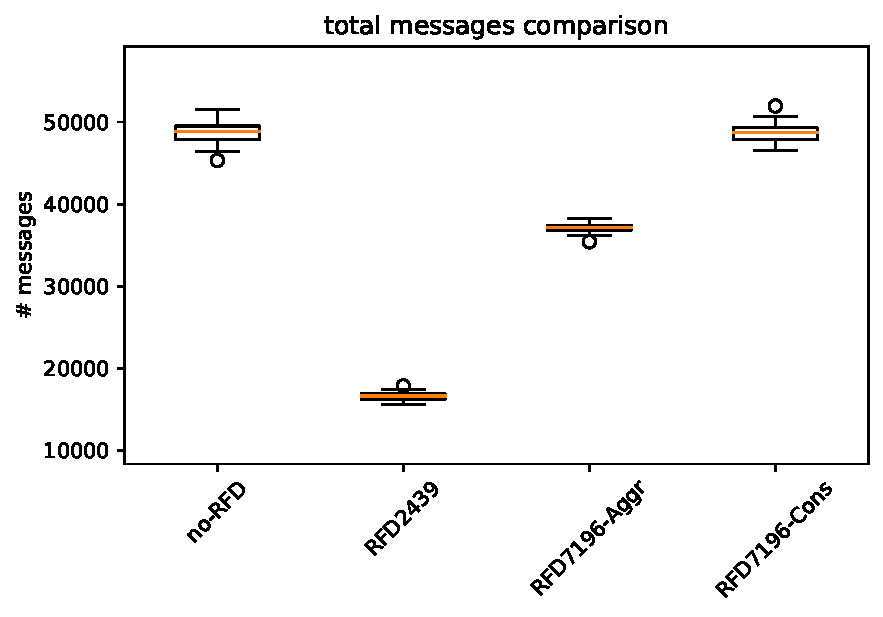
\includegraphics[width=\textwidth]{images/RFD/miceVSelephants/mice/cisco_1000MRAI30_rfd_comparison_messages_boxplot.pdf}
         \caption{Number of messages respect to the RFD strategy}
         \label{fig:1000_RFD_MRAI30_mice_messages}
     \end{subfigure}
     \hfill
     \begin{subfigure}[b]{0.325\textwidth}
         \centering
         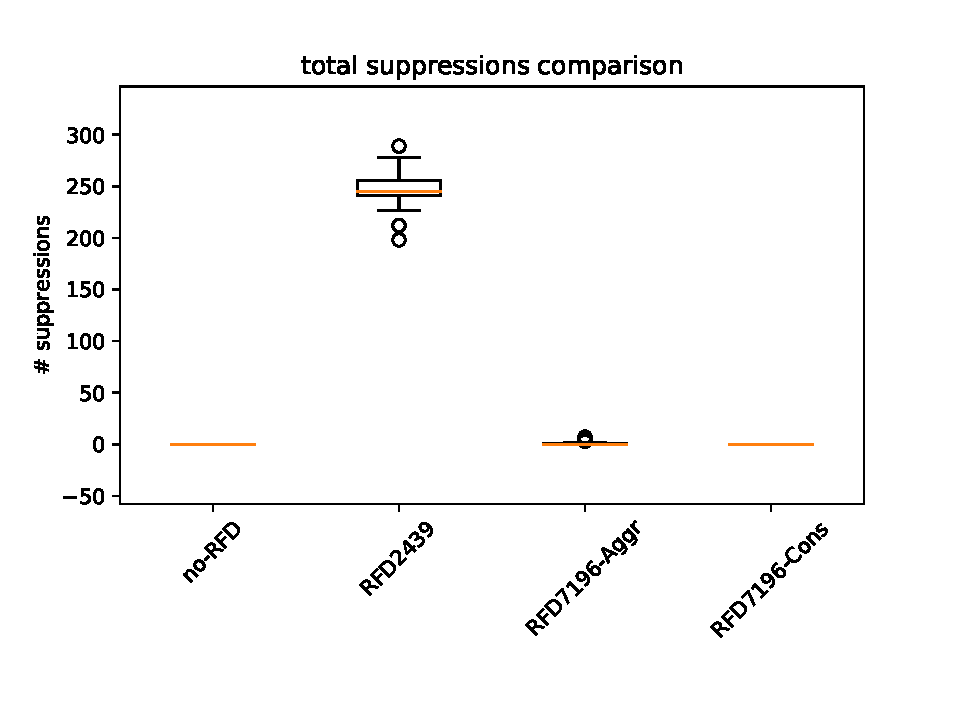
\includegraphics[width=\textwidth]{images/RFD/miceVSelephants/mice/cisco_1000MRAI30_rfd_comparison_suppressions_boxplot.pdf}
         \caption{Number of suppressions respect to the RFD strategy}
         \label{fig:1000_RFD_MRAI30_mice_suppressions}
     \end{subfigure}
		\caption{Internet like topology 1000 nodes, MRAI=30s, random destination, 5 flaps, \SI{300}{\second} message delay, Network performances}
        \label{fig:1000_RFD_MRAI30_mice}
\end{figure}

From \Cref{fig:1000_RFD_MRAI30_mice_suppressions} we can see that there is a
big difference in terms of suppressions.
The standard strategy produces on average \num{250} suppressions and the effects
of those suppressions can be sawed in \Cref{fig:1000_RFD_MRAI30_mice_time} because its
the only strategy that on average has a convergence time higher than \SI{4500}{\second}
The opposite case is represented by the \textit{Conservative} from \ac{RFC} 7196
\cite{rfc7196}.
The threshold in this last case is so permissive that  it doesn't have any effect
different the \textit{NoRFD} strategy.
In the middle, we find the \textit{Aggressive} strategy, in \Cref{fig:1000_RFD_MRAI30_mice_suppressions}
we can see that on average it doesn't suppress anything, but it can happen that
it produces few suppressions.
The effects of those suppressions are visible in \Cref{fig:1000_RFD_MRAI30_mice_time}
where, with this strategy is possible to have a very huge convergence time, caused
by the fact that it takes more time to recover from a route that overpass a threshold
of \num{6.0} in respect of \num{2.0}.
In \Cref{fig:1000_RFD_MRAI30_mice_messages} we can see that the number of messages
transmitted is distribute as expected, the two more permissive strategies have the
same behaviour of the \textit{NoRFD} while the standard strategy never produces
more than \num{8000} messages.

We can then study which are the nodes that produce the suppressions and how
far are them from the signal source.
We can see the results of this study, for each suppression technique in \Cref{fig:1000_RFD_centVSsup}.

\begin{figure}[h]
     \centering
     \begin{subfigure}[b]{0.325\textwidth}
         \centering
         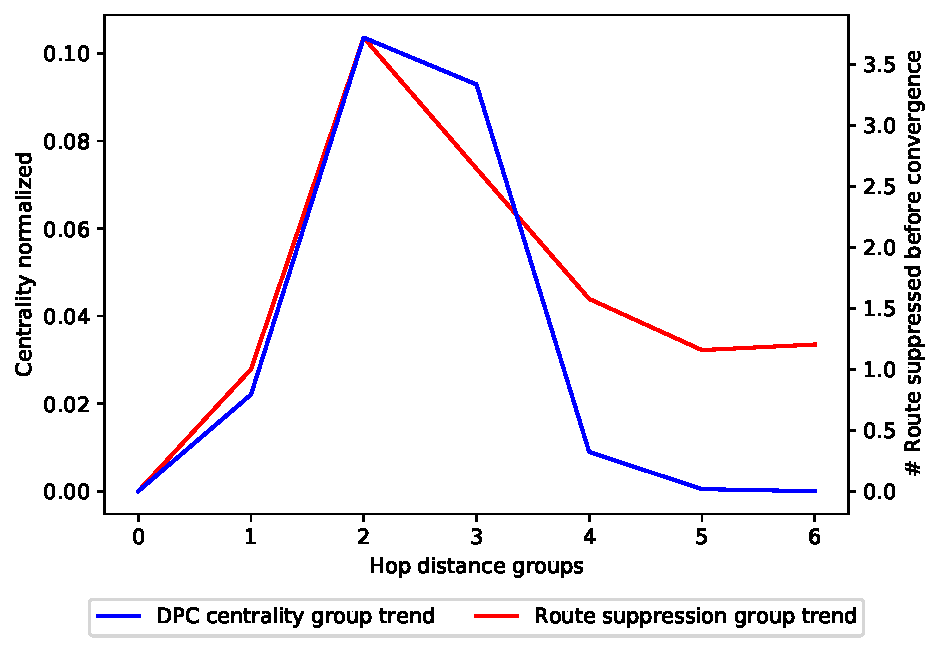
\includegraphics[width=\textwidth]{images/RFD/miceVSelephants/mice/cisco_1000_RFD_nodeConvergence_centVSsup_trend.pdf}
         \caption{RFD 2439 Strategy}
         \label{fig:1000_2439RFD_centVSsup}
     \end{subfigure}
     \hfill
     \begin{subfigure}[b]{0.325\textwidth}
         \centering
         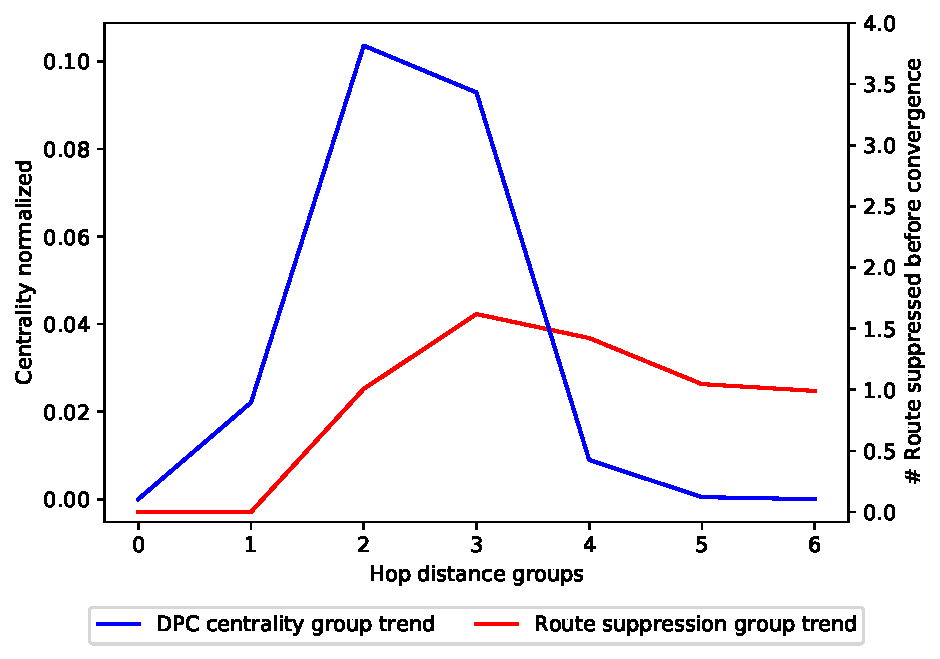
\includegraphics[width=\textwidth]{images/RFD/miceVSelephants/mice/cisco_1000_RFD_7196_aggressive_nodeConvergence_centVSsup_trend.pdf}
         \caption{RFD 7196 Aggressive Strategy}
         \label{fig:1000_7196RFDA_centVSsup}
     \end{subfigure}
     \hfill
     \begin{subfigure}[b]{0.325\textwidth}
         \centering
         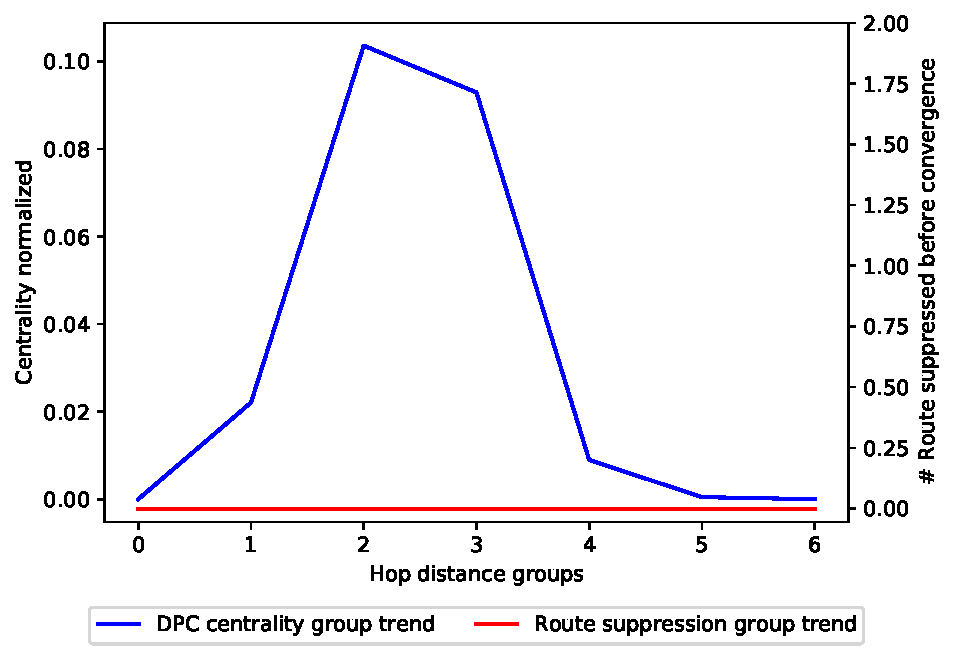
\includegraphics[width=\textwidth]{images/RFD/miceVSelephants/mice/cisco_1000_RFD_7196_conservative_nodeConvergence_centVSsup_trend.pdf}
         \caption{RFD 7196 Conservative Strategy}
         \label{fig:1000_7196RFDC_centVSsup}
     \end{subfigure}
		\caption{Internet like topology \num{1000} nodes, \ac{MRAI} = \SI{30}{\second}, random destination, \num{5} flaps, \SI{300}{\second} between messages, Suppression trend VS avg hop centrality}
        \label{fig:1000_RFD_centVSsup}
\end{figure}

For the plots in \Cref{fig:1000_RFD_centVSsup} the $x$ axis represent the distance
from the source node in terms of hops and all the other nodes are grouped by this
distance.
The blue line represents the average centrality of the groups, for each node of the
graph I calculated the centrality using the \ac{DPC} metric then grouped them
and calculated the average value.
As expected the central nodes have a higher centrality and them are at few hops
of distance
from the source node.
The centrality trend is equal for each plot in \Cref{fig:1000_RFD_centVSsup}
because the graph and the source node are the same for each experiment.

The red line represents the average number of suppressions per group.
As we can see with the standard strategy, \Cref{fig:1000_2439RFD_centVSsup}, 
on average, the route is blocked \num{2} times be the nearest nodes and then, 
this value slowly decreases in the following groups but it will be still
blocked a few times in the farthest nodes.
The \textit{Aggressive} strategy, \Cref{fig:1000_7196RFDA_centVSsup} present
a completely different behaviour, the nearest nodes blocks a few times the 
route, while the most central nodes almost never and the farthest nodes never
blocks it.
This is meaningful because it tells us that the few suppressions in the nearest
nodes are enough to not trigger other blocks in the next groups.
As expected with the \textit{Conservative} strategy we don't have suppressions at
all.

\subsection{Elephants}
\label{subsec:bgp_elephants}

The elephants prefixes, as I mentioned in \Cref{sec:bgp_rfd_mice_vs_elephants},
are the ones that produce the majority of the \ac{ADV}.
And we also know, thanks to \cite{huston2006bgp}, that is possible to see over
thousands of messages per day.
For this reason, the \textit{elephants} environment signal is composed by \num{100}
flaps, with a delay between the messages of \SI{3}{\second}.
All the other properties of the environment are unchanged.
The results are presented in \Cref{fig:1000_RFD_MRAI30_elephant,fig:1000_RFD_centVSsup_elephants}.

\begin{figure}[h]
     \centering
     \begin{subfigure}[b]{0.325\textwidth}
         \centering
         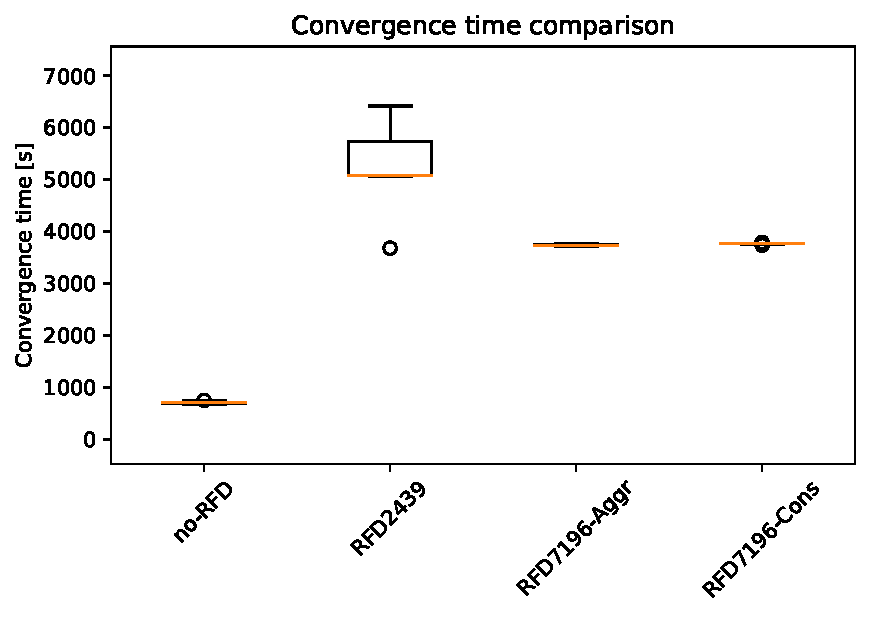
\includegraphics[width=\textwidth]{images/RFD/miceVSelephants/elephants/cisco_1000MRAI30_rfd_comparison_time_boxplot.pdf}
         \caption{Convergence time respect to the RFD strategy}
         \label{fig:1000_RFD_MRAI30_time_elephant}
     \end{subfigure}
     \hfill
     \begin{subfigure}[b]{0.325\textwidth}
         \centering
         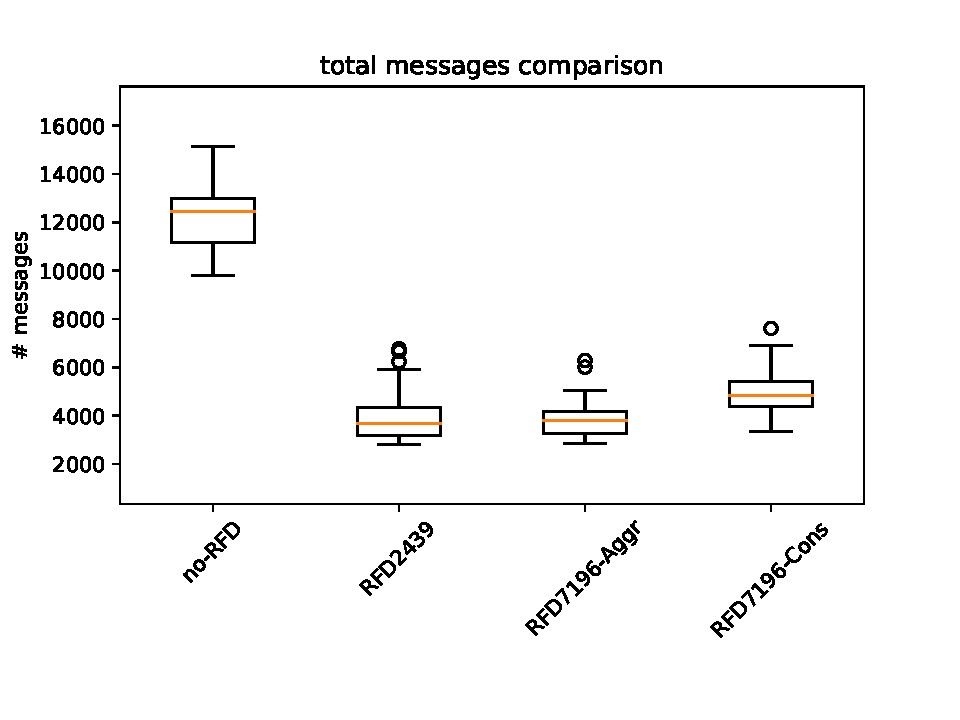
\includegraphics[width=\textwidth]{images/RFD/miceVSelephants/elephants/cisco_1000MRAI30_rfd_comparison_messages_boxplot.pdf}
         \caption{Number of messages respect to the RFD strategy}
         \label{fig:1000_RFD_MRAI30_messages_elephant}
     \end{subfigure}
     \hfill
     \begin{subfigure}[b]{0.325\textwidth}
         \centering
         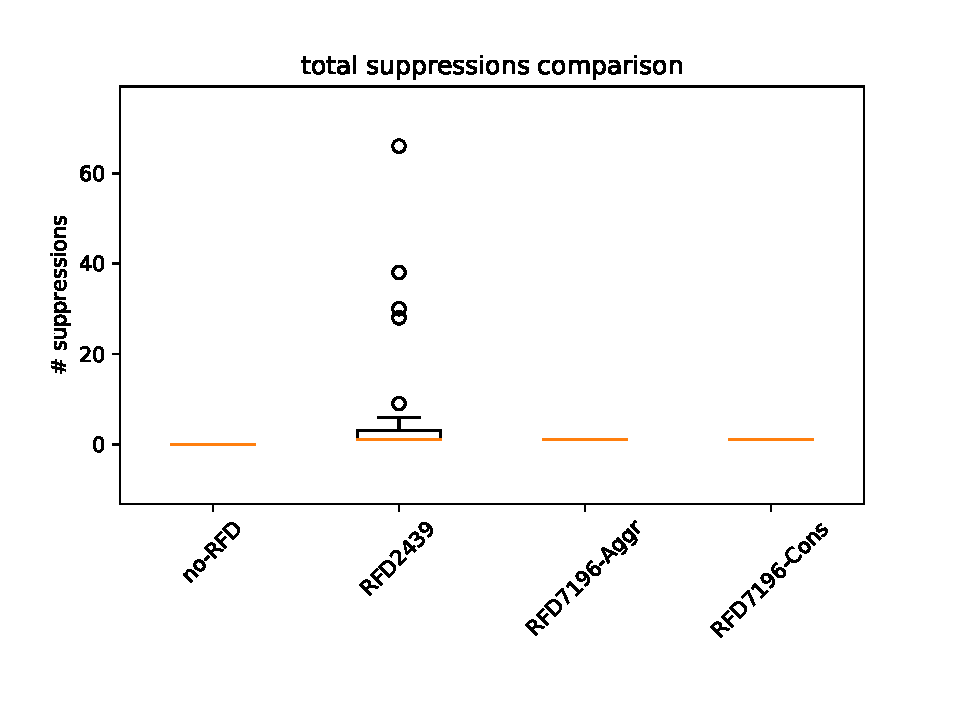
\includegraphics[width=\textwidth]{images/RFD/miceVSelephants/elephants/cisco_1000MRAI30_rfd_comparison_suppressions_boxplot.pdf}
         \caption{Number of suppressions respect to the RFD strategy}
         \label{fig:1000_RFD_MRAI30_suppressions_elephant}
     \end{subfigure}
		\caption{Internet like topology \num{1000} nodes, \ac{MRAI} = \SI{30}{\second}, random destination, \num{100} flaps, \SI{3}{\second} delay, Network performances}
        \label{fig:1000_RFD_MRAI30_elephant}
\end{figure}

Is possible to see in \Cref{fig:1000_RFD_MRAI30_elephant} that this time we have
a different behaviour from all the \num{3} \ac{RFD} strategies.
In \Cref{fig:1000_RFD_MRAI30_suppressions_elephant} we can see that the
standard strategy doesn't have any more hundreds of suppressions, but on average
ti suppress few times the route and this is sufficient.
The same behaviour, with less variance, is obtained from the \textit{Aggressive}
and \textit{Conservative} strategies.
Also in \Cref{fig:1000_RFD_MRAI30_messages_elephant,fig:1000_RFD_MRAI30_time_elephant}
we can notice a similar trend, the three strategies react in the same way,
producing a smaller number of messages (on average $1/3$) in respect of the 
\textit{NoRFD} strategy.

\begin{figure}[H]
     \centering
     \begin{subfigure}[b]{0.325\textwidth}
         \centering
         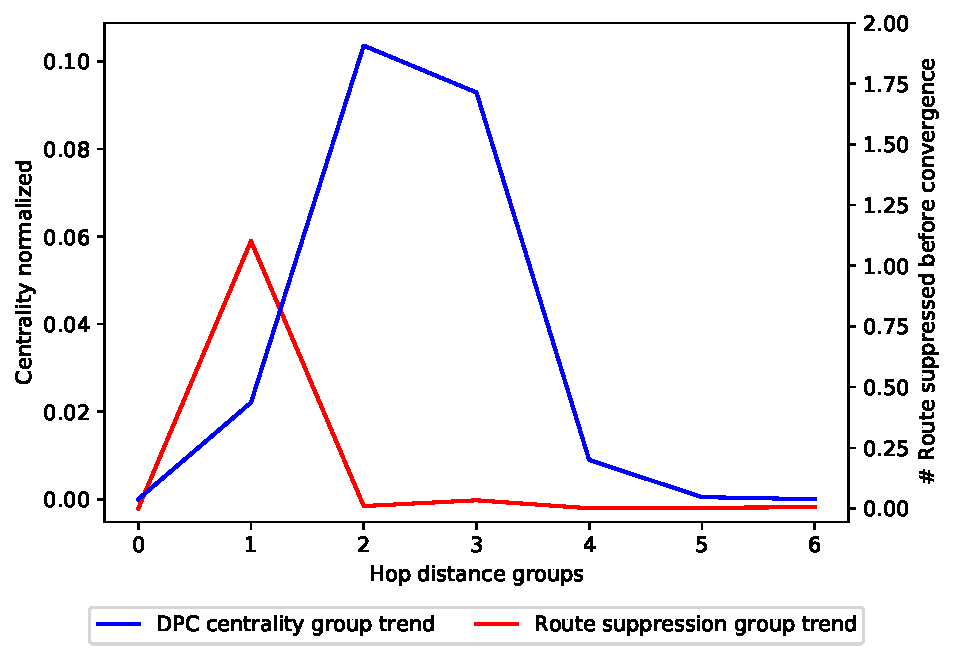
\includegraphics[width=\textwidth]{images/RFD/miceVSelephants/elephants/cisco_1000_RFD_nodeConvergence_centVSsup_trend.pdf}
         \caption{RFD 2439 Strategy}
         \label{fig:1000_2439RFD_centVSsup_elephants}
     \end{subfigure}
     \hfill
     \begin{subfigure}[b]{0.325\textwidth}
         \centering
         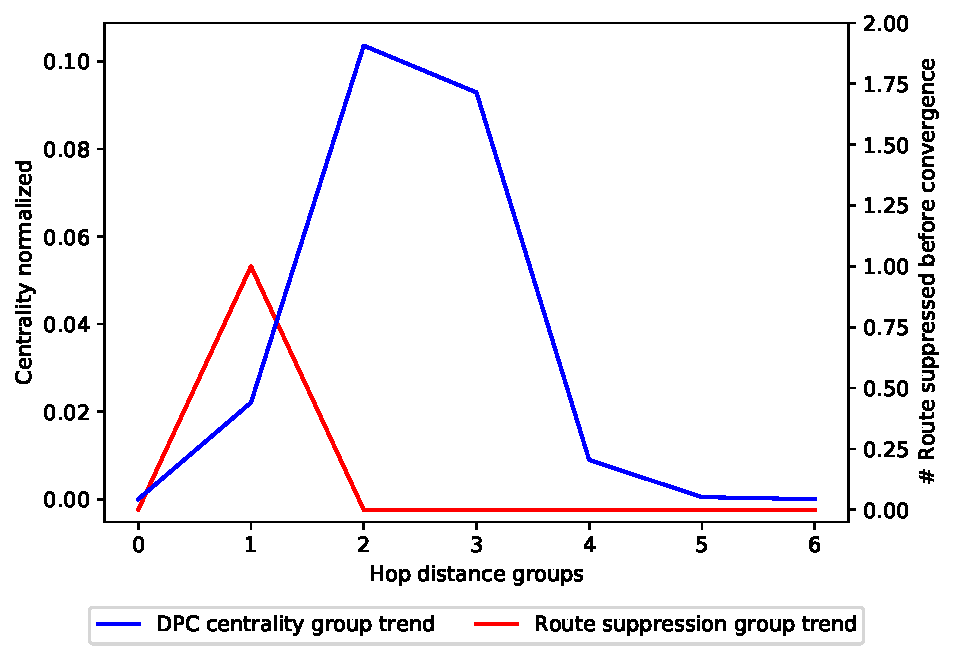
\includegraphics[width=\textwidth]{images/RFD/miceVSelephants/elephants/cisco_1000_RFD_7196_aggressive_nodeConvergence_centVSsup_trend.pdf}
         \caption{RFD 7196 Aggressive Strategy}
         \label{fig:1000_7196RFDA_centVSsup_elephants}
     \end{subfigure}
     \hfill
     \begin{subfigure}[b]{0.325\textwidth}
         \centering
         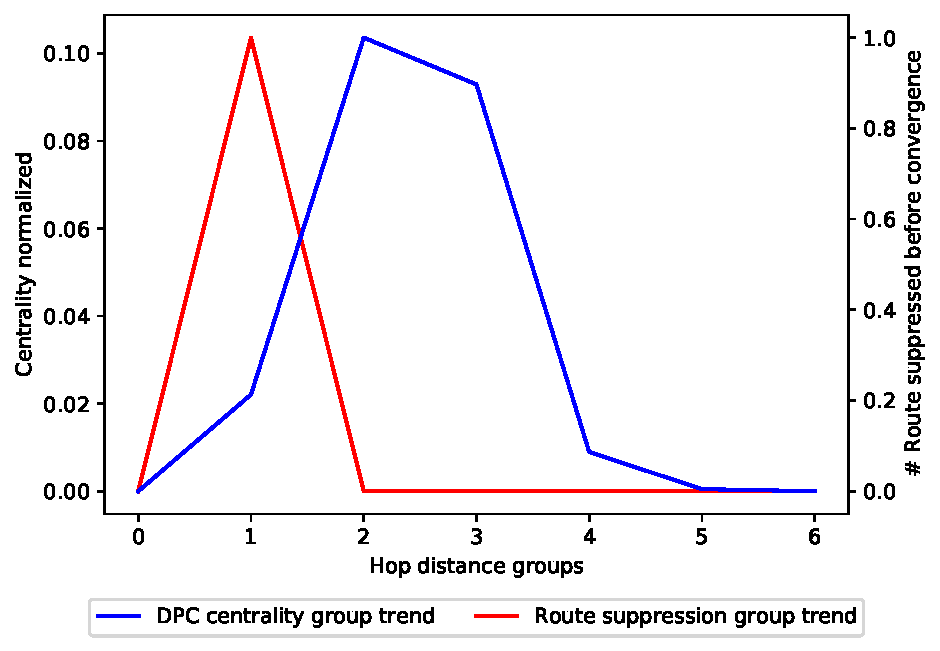
\includegraphics[width=\textwidth]{images/RFD/miceVSelephants/elephants/cisco_1000_RFD_7196_conservative_nodeConvergence_centVSsup_trend.pdf}
         \caption{RFD 7196 Conservative Strategy}
         \label{fig:1000_7196RFDC_centVSsup_elephants}
     \end{subfigure}
		\caption{Internet like topology \num{1000} nodes, \ac{MRAI} = \SI{30}{\second}, random destination, \num{100} flaps, \SI{3}{\second} delay, Network performances}
        \label{fig:1000_RFD_centVSsup_elephants}
\end{figure}

The same trend can be saw in \Cref{fig:1000_RFD_centVSsup_elephants}, were
the three strategies produce on average one single suppression in the nearest
group.

We can then say that all the strategies catch in time the flap and avoid the
propagation of the update storm, increasing the convergence time but protecting 
the network from thousands of messages.

\subsection{MRAI influence on Mice and Elephants}
\label{subsec:bgp_rfd_mrai_influence_mice_elephants}

We can now study the influence of \ac{MRAI} on those two cases.
The environments are equal to the previous section.
The results of the \textit{Mice} case are exposed in \Cref{fig:1000_RFD_multiMRAI_mice},
while the results of the elephant case are in \Cref{fig:1000_RFD_multiMRAI_elephants}.

\begin{figure}[h]
     \centering
     \begin{subfigure}[b]{0.325\textwidth}
         \centering
         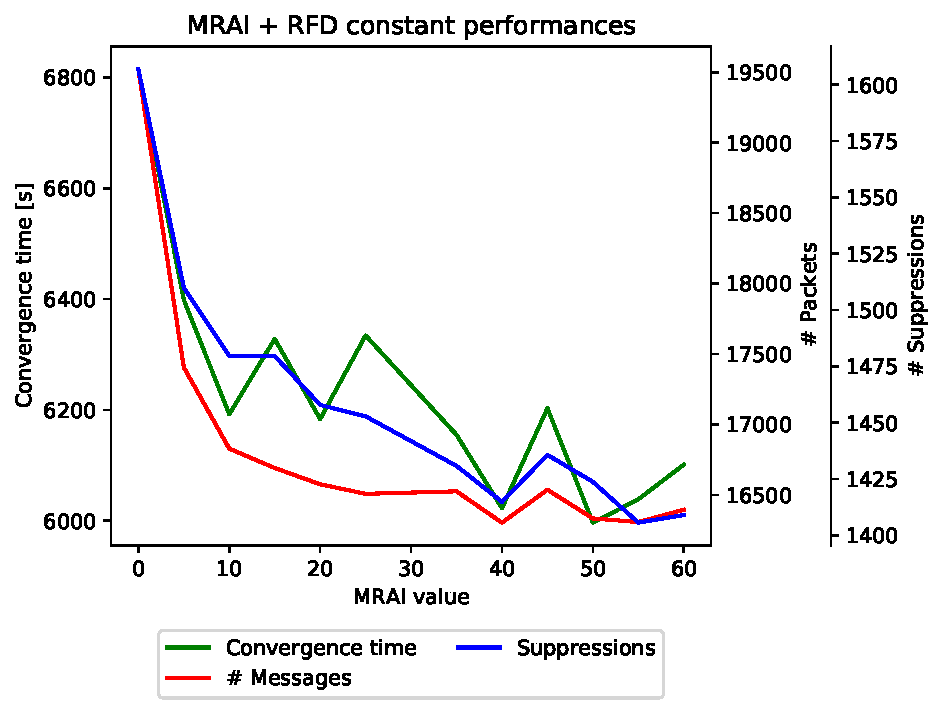
\includegraphics[width=\textwidth]{images/RFD/miceVSelephants/MultiMRAI/mice/cisco_1000_RFD_2439-constant_mrai_rfd_evolution.pdf}
         \caption{RFD 2439 Strategy}
         \label{fig:1000_2439RFD_multiMRAI_mice}
     \end{subfigure}
     \hfill
     \begin{subfigure}[b]{0.325\textwidth}
         \centering
         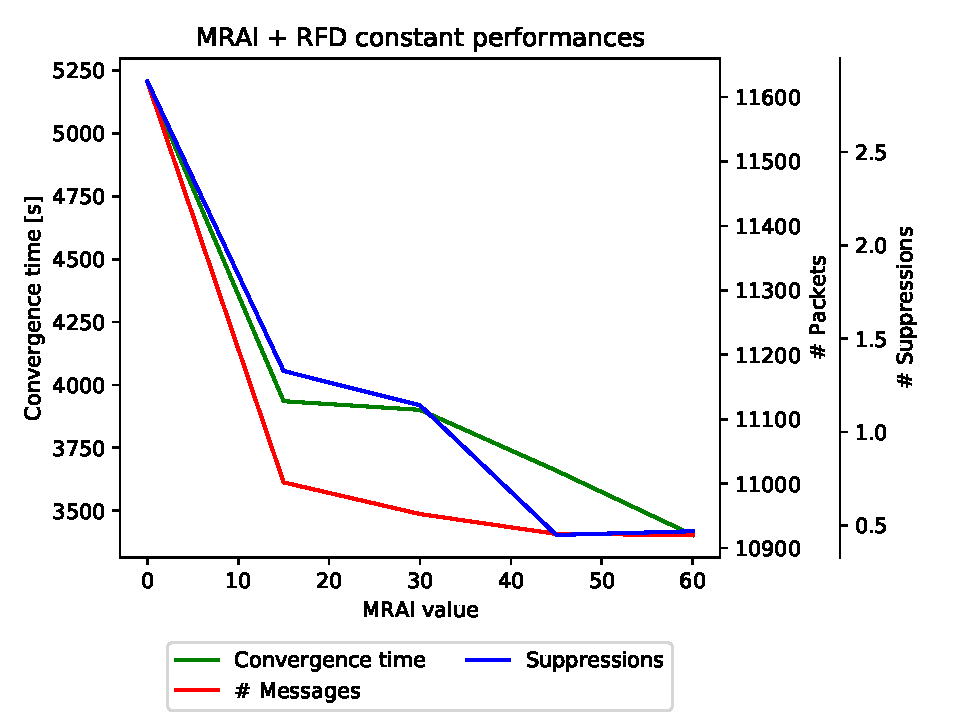
\includegraphics[width=\textwidth]{images/RFD/miceVSelephants/MultiMRAI/mice/cisco_1000_RFD_7196_aggressive-constant_mrai_rfd_evolution.pdf}
         \caption{RFD 7196 Aggressive Strategy}
         \label{fig:1000_7196RFDA_multiMRAI_mice}
     \end{subfigure}
     \hfill
     \begin{subfigure}[b]{0.325\textwidth}
         \centering
         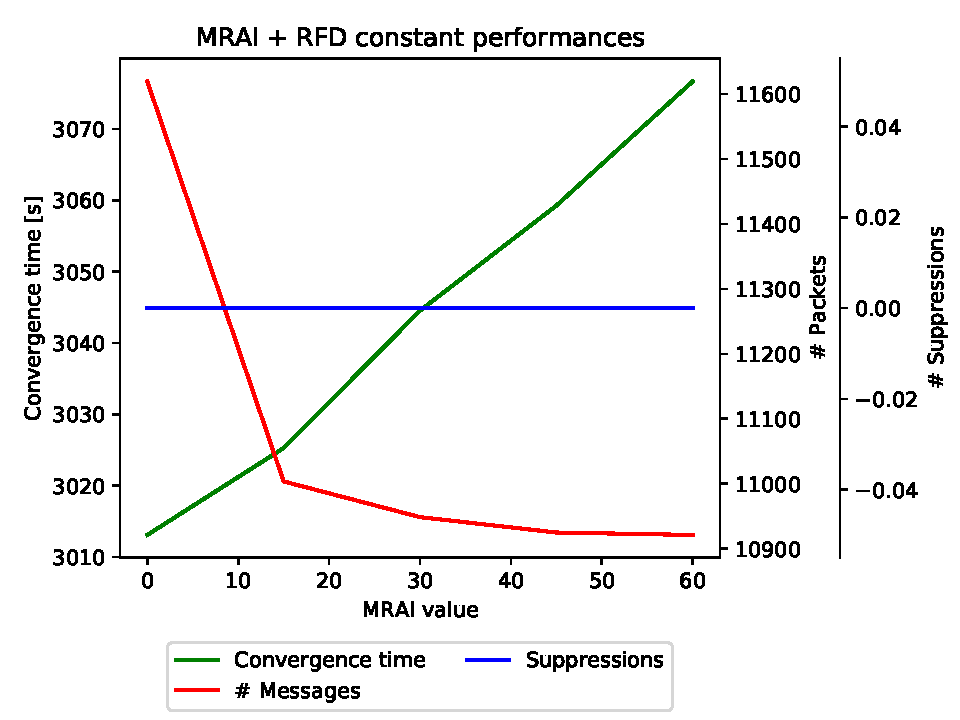
\includegraphics[width=\textwidth]{images/RFD/miceVSelephants/MultiMRAI/mice/cisco_1000_RFD_7196_conservative-constant_mrai_rfd_evolution.pdf}
         \caption{RFD 7196 Conservative Strategy}
         \label{fig:1000_7196RFDC_multiMRAI_mice}
     \end{subfigure}
		\caption{Internet like topology \num{1000} nodes, random destination, \num{100} flaps, \SI{3}{\second} delay, Network performances}
        \label{fig:1000_RFD_multiMRAI_mice}
\end{figure}

\fxfatal{I don't really know how to explain the RFD curve in \Cref{fig:1000_2439RFD_multiMRAI_mice}}

\begin{figure}[h]
     \centering
     \begin{subfigure}[b]{0.325\textwidth}
         \centering
         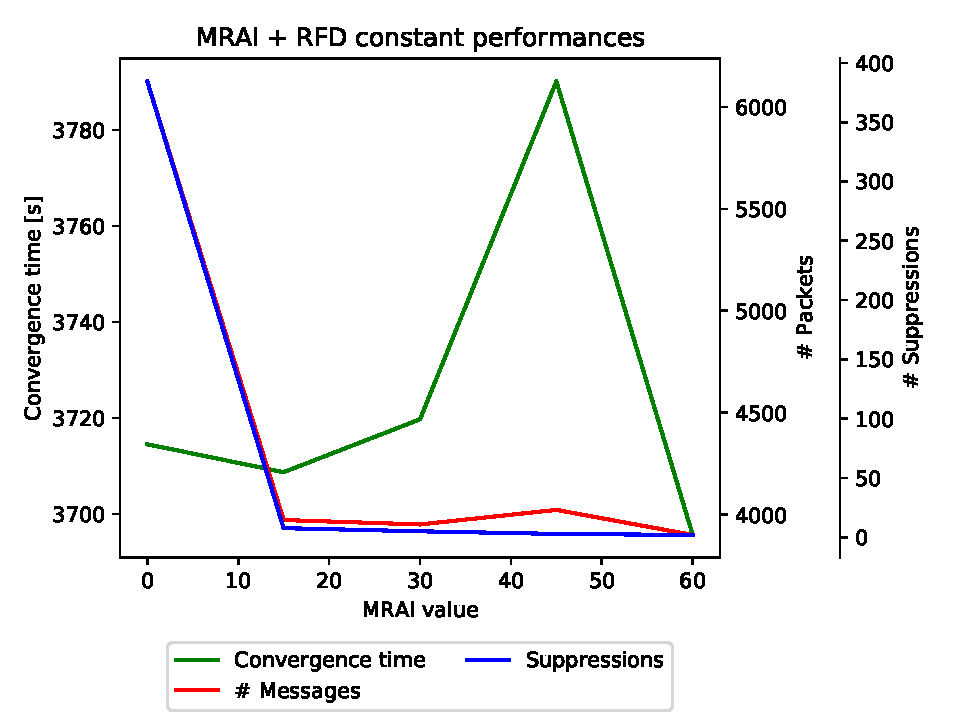
\includegraphics[width=\textwidth]{images/RFD/miceVSelephants/MultiMRAI/elephants/cisco_1000_RFD_2439-constant_mrai_rfd_evolution.pdf}
         \caption{RFD 2439 Strategy}
         \label{fig:1000_2439RFD_multiMRAI_elephants}
     \end{subfigure}
     \hfill
     \begin{subfigure}[b]{0.325\textwidth}
         \centering
         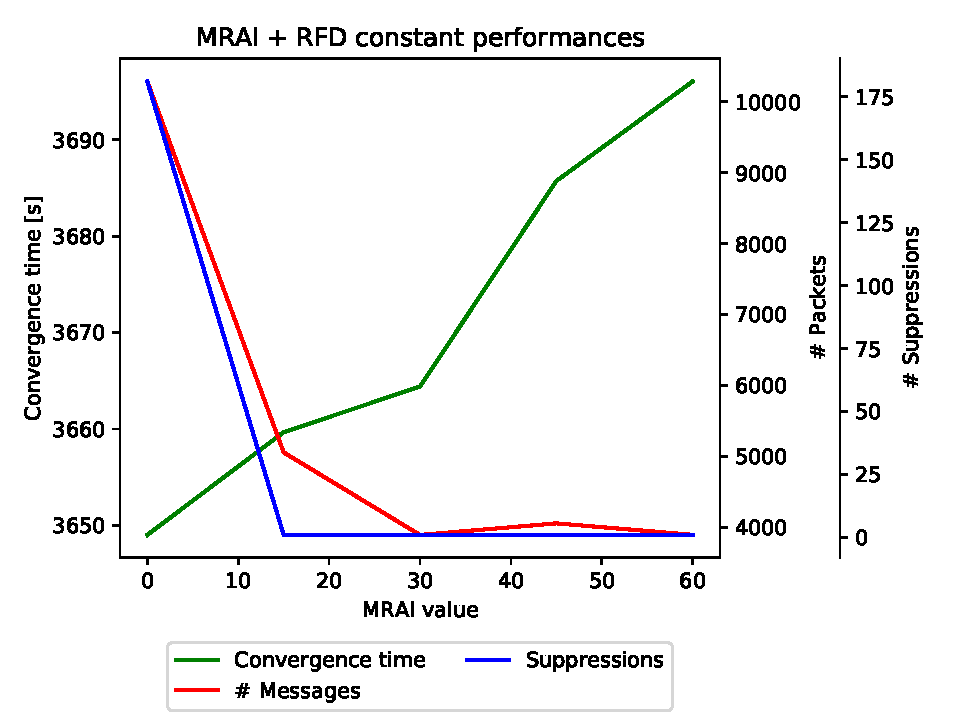
\includegraphics[width=\textwidth]{images/RFD/miceVSelephants/MultiMRAI/elephants/cisco_1000_RFD_7196_aggressive-constant_mrai_rfd_evolution.pdf}
         \caption{RFD 7196 Aggressive Strategy}
         \label{fig:1000_7196RFDA_multiMRAI_elephants}
     \end{subfigure}
     \hfill
     \begin{subfigure}[b]{0.325\textwidth}
         \centering
         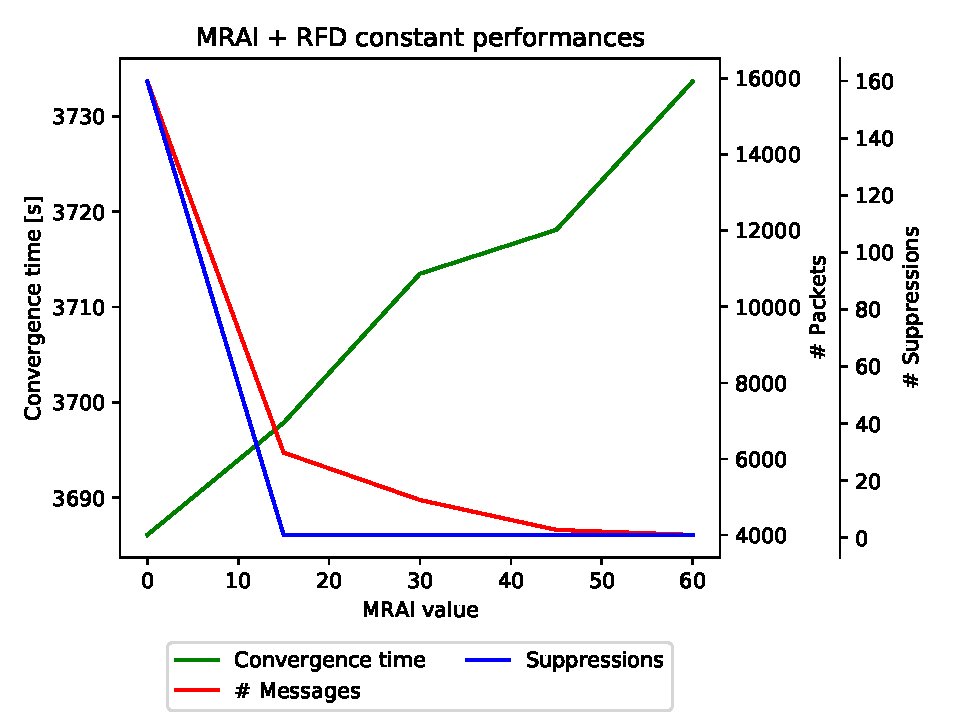
\includegraphics[width=\textwidth]{images/RFD/miceVSelephants/MultiMRAI/elephants/cisco_1000_RFD_7196_conservative-constant_mrai_rfd_evolution.pdf}
         \caption{RFD 7196 Conservative Strategy}
         \label{fig:1000_7196RFDC_multiMRAI_elephants}
     \end{subfigure}
		\caption{Internet like topology \num{1000} nodes, random destination, \num{100} flaps, \SI{3}{\second} delay, Network performances}
        \label{fig:1000_RFD_multiMRAI_elephants}
\end{figure}

The boxplots that shows the evolution comparing the different strategy are
in the \Cref{cha:appendx}

%\begin{itemize}
%    \item What is Mice VS Elephants?
%    \item How has been studied in the past?
%    \item Introduce how MRAI affects mice VS elephants
%\end{itemize}
